\documentclass[a4paper,12pt]{report}
\usepackage[utf8x]{inputenc}
\usepackage[T1]{fontenc}
\usepackage[french]{babel}
\usepackage[superscript,biblabel]{cite}	% Références en indice
\usepackage[justification=centering]{caption} % Centrer les légendes
\usepackage[hyphenbreaks]{breakurl}
\usepackage[hyphens]{url}
\usepackage{graphicx,eso-pic,eurosym,tabularx,hyperref,setspace,fullpage}

\hypersetup{
    colorlinks=true,                         
    citecolor=blue, % Couleur des numéros de la biblio dans le corps
   	urlcolor=blue,   % Couleur des url
   	linkcolor=black}  % Couleur des liens internes


\newcolumntype{M}[1]{>{\centering\arraybackslash}m{#1}} %Nouveau style de colone pour le tableau de Flavien

\newcommand\BackgroundPic{				%Fond avec le logo INSA
	\put(0,250){
		\parbox[b][\paperheight]{\paperwidth}{
			\vfill
			\centering
			
\includegraphics[width=\paperwidth,height=\paperheight,keepaspectratio]{logoINSA.jpg}
			\vfill
}}}

\onehalfspacing %interline 1.5

\title{La place de l'innovation dans l'économie bretonne}
\author{ \bsc{Aurélien Fontaine}
	\and \bsc{Manutea Huang} 
	\and \bsc{Nicolas Le Borgne}
	\and \bsc{Maxime Cadoret}
	\and \bsc{Flavien Lecuyer}
}
\date{\today}



\begin{document}
	\AddToShipoutPicture*{\BackgroundPic}
	\maketitle

	\chapter*{Remerciements}
	Nous souhaitons tout d'abord remercier l'équipe de Valorial pour leur disponibilité ainsi que pour leurs informations précieuses.
	
	Nous voudrions également remercier Monsieur Simon LE BAYON pour son apport de connaissances.

	Nous aimerions remercier Madame Hélène PRIGENT pour son aide et son soutien lors de l'écriture de cette monographie.
	
	\setcounter{tocdepth}{2}
	\tableofcontents
	
\chapter*{Introduction}
\addcontentsline{toc}{chapter}{Introduction}
	 L’industrie agro-alimentaire tient depuis longtemps une place prépondérante dans l’économie bretonne. En effet, celle-ci représente plus de 40\% du secteur industriel régional ainsi que 15\% de la valeur ajoutée créée pour ce secteur au niveau national. 
	 
	 L’importance de l’agro-alimentaire dans le tissu économique breton donne d’ailleurs à la région une image très rurale, laquelle tend s'ancrer tant l’évolution de ce secteur est significative. Malgré la baisse conséquente du nombre de salariés dans le secteur manufacturier entre 2010 et 2012, qui ont ainsi été réduit de 42\%, l’agro-alimentaire reste la principale source d’emploi dans la région. La part de l’agro-alimentaire dans la masse salariale de l’industrie manufacturière est passée à près de deux emplois sur trois (de 37\% à 62\%) dans la même période.
	 
	 Malgré tout, l’économie agro-alimentaire ne garde qu’une importance faible dans l’apport de richesses au territoire local. La prédominance des industries de première transformation provoque ainsi une baisse des taux de valeur ajoutée par rapport à la moyenne nationale des IAA (Industries Agro-Alimentaires). Cela fragilise ainsi cette économie, qui doit donc réduire les prix afin de rester compétitive face aux marchés étrangers tout en étant fragilisée par les lois françaises de plus en plus strictes. A titre d’exemple, les années 2012 et 2013 ont été marquées par des restructurations importantes touchant essentiellement le secteur de l’abattage et de la première transformation. Ces restructurations, qui pourraient se poursuivre, ont eu des conséquences sur l’emploi dans des territoires fragilisés, notamment dans le Morbihan et dans le Finistère. Les difficultés subies dans l’agro-alimentaire, en particulier pour les filières porcines et volaillères, ont créé des réactions en chaîne, qui ont de ce fait dépassé le cadre de l’agro-alimentaire.
	 
	 Dans le but de mieux répondre à ces problèmes, on constate de la part des entreprises une volonté forte de se diversifier au travers de l’innovation. En l’espace de dix ans, les industriels ont ainsi réussi à mettre en place de nouvelles gammes de produits, permettant donc d’augmenter leur taux de valeur ajoutée et par extension placer la Bretagne à la première place en termes de valeur ajoutée dans le classement français selon le gouvernement. Pourtant, l'innovation reste un phénomène trop peu fréquent, comme en atteste le peu de changement dans les rayons de supermarchés. On remarque ainsi un manque cruel d'entreprises innovantes dans le secteur.
	 
	 Cela donne par conséquent une place spécifique aux problèmes de l'innovation dans l’économie bretonne. Nous pouvons ainsi nous demander « Quelle est la place de l'innovation de l'industrie agro-alimentaire bretonne et comment peut-elle évoluer ? » Afin de répondre à cette question, nous nous intéresserons de prime abord à la situation de l’agro-alimentaire dans la région Bretagne. Dans un second temps, nous présenterons les avantages que tirent les entreprises de l'innovation. Pour finir, nous nous pencherons sur les problèmes que cela pose et sur les nouvelles perspectives d'innovation. Dans ce développement, nous nous pencherons également sur le cas de Valorial qui représente bien la situation actuelle.
	 
\chapter{La situation agro-alimentaire bretonne}
	Aujourd’hui, et depuis quelques années, la situation de l’industrie agro-alimentaire tend à se dégrader à l’international. Pour autant, la Bretagne semble bien s’en sortir, comme en attestent les chiffres. Cela rend donc la situation de cette industrie particulière. Afin de la présenter en détail, nous commencerons par voir la situation de l’agro-alimentaire français à l’international. Ensuite, nous comparerons la situation de la Bretagne à celle de la France. Pour finir, nous parlerons de la crise dans l’agro-alimentaire et des actions menées pour la gérer.

	\section{L’agro-alimentaire français dans le marché international}
		Comme beaucoup le savent, l’agro-alimentaire est dans une situation peu avantageuse depuis quelques années, affaiblie par plusieurs crises en quelques années. Afin de donner un état des lieux de cette industrie, nous verrons tout d’abord les problèmes qu’ont les entreprises à conserver leur compétitivité. Dans un second temps, nous nous intéresserons aux problèmes de l’emploi dans le secteur. Pour finir, nous verrons que ce mauvais bilan se rattrape au travers de la technologie et de l’export.

		\subsection{La compétitivité en baisse}
			Pour commencer, on remarque que la compétitivité de l’industrie agro-alimentaire est dans une tendance à la baisse.
			
			Au cours des années 2000, la France était le premier exportateur agro-alimentaire européen. Aujourd'hui l’Allemagne et les Pays-Bas sont passés devant la France qui se place en troisième position, et il arrive que certains secteurs de l’industrie agro-alimentaire comme celui de la viande aient une balance commerciale déficitaire : “le déficit commercial s'est creusé de 20\% au 2e trimestre 2013 sur un an”\cite{DeficitCommercialViandeAggrave}.

			Ce recul de la France est dû, entre autres, aux nombreux obstacles qui “freinent le développement de cette industrie”\cite{StimulerCompetitiviteEntreprises}. Ils sont d’ordres multiples. Par exemple, il y a une certaine difficulté à recruter de nouveaux employés, plus particulièrement des personnes qualifiées. Le secteur de l’agro-alimentaire n’est pas très attirant suite à la croissance du monde numérique mais nécessite une grande main d’oeuvre.

			De plus, les investisseurs comme les banques ou les grands groupes sont de moins en moins enclins à accorder des fonds aux entreprises. Or le coût des matières premières ne cesse de croître alors que les prix pour le client final stagnent. Les entreprises ont donc une marge de manœuvre de plus en plus réduite pour développer de nouvelles méthodes. De surcroît, la législation française est très contraignante. En effet, aujourd’hui les consommateurs sont de plus en plus critiques vis-à-vis du produit : pour eux, la sécurité et la qualité alimentaire sont tout aussi importants que l’aspect diététique ou énergétique du produit qu’ils consomment. De ce fait, une traçabilité parfaite doit être mise en place afin de plaire aux consommateurs. “Cet impératif est lourd financièrement, surtout dans un environnement économique, social et réglementaire très hétérogène”\cite{SecteurAAFrancaisEnjeuxXXISiecle}. Cette hétérogénéité vient du fait des différentes loi sanitaires en Europe, et encore plus dans le monde, ce qui pose de nombreux problèmes pour les entreprises agro-alimentaires françaises qui sont soumises à des lois bien plus contraignantes que celles du reste du monde. Si l’on prend l’exemple du marché de la volaille : le Brésil vient de se hisser au premier rang mondial d’exportateur de volailles devant les États-Unis et l’Europe. Cette ascension est due au modèle économique du Brésil vis-à-vis de ce marché qui ne cesse de croître, les banques doivent permettre aux exploitants de volailles d'emprunter à faible taux. Ces faibles taux permettent un investissement conséquent et une baisse les prix de vente. Face au Brésil, les subventions se font de plus en plus rares notamment avec “la fin des aides à l'export [...] en juillet, qui soutenaient la filière à hauteur de 55 millions d'euros par an”.\cite{PouletBresilienMoinsCherBreton} Ces deux phénomènes cumulés font perdre depuis dix ans des parts de marché à deux grands volaillers bretons (Doux et Tilly-Sabco) .
			

		\subsection{Le paradoxe de la productivité et de l'emploi}
			Pour ce qui est de l’emploi, on constate aujourd'hui un paradoxe important. En effet, les industriels de l’industrie agro-alimentaire sont de plus en plus productifs, mais on se heurte en parallèle avec une baisse de plus en plus conséquente du nombre d’emplois et d’organisations dans le secteur.
			
			Certains moyens ont été mis en place afin d’aider les entreprises comme des sites de recrutement sur internet : \url{www.jobagroalimentaire.com} ou \url{www.apecita.com} .  “Ces mauvais indices surviennent dans un contexte de baisse de la production de 2,6\% du secteur [de la viande]. Ce climat pèse bien sûr sur l'emploi puisque la filière a perdu 7.200 emplois entre juin 2013 et juin 2012”\cite{DeficitCommercialViandeAggrave}.
			
			Le secteur de l’agro-alimentaire a de moins en moins d’employés. En effet, en 10 ans, le nombre d’employés dans ce secteur a baissé de 4000\cite{IAAHeritageAgricoleBretagne} et pourtant on peut voir une hausse de la production de ce secteur : entre 2005 et 2012, le volume des productions européennes a progressé de 4\%\cite{HausseModereeVenteProduitsAA2012}. Néanmoins, lors du premier semestre 2014, la production dans le secteur de l’agro-alimentaire a reculé de 2,2\% là où l’année précédent il y avait eu une augmentation de 0,6\%\cite{ReculHistoriqueProductionAAFrance}. Ceci est une première dans l’histoire française
			
			Il y a certaines innovations qui sont très fortement critiquées comme la Ferme des milles vaches située dans la Somme\cite{Ferme1000Vaches}. Elle s'inspire des grandes fermes allemandes ou hollandaises qui ont fait ce choix par manque de place. En effet, cette ferme boulverse les conventions des agriculteurs français et de l'élevage familial, avec des petits troupeaux qui reste d’une taille modeste (actuellement, moins de la moitié des troupeaux français dépasse les 50 bovins).
			
			\begin{figure}[!h]
				\centering
				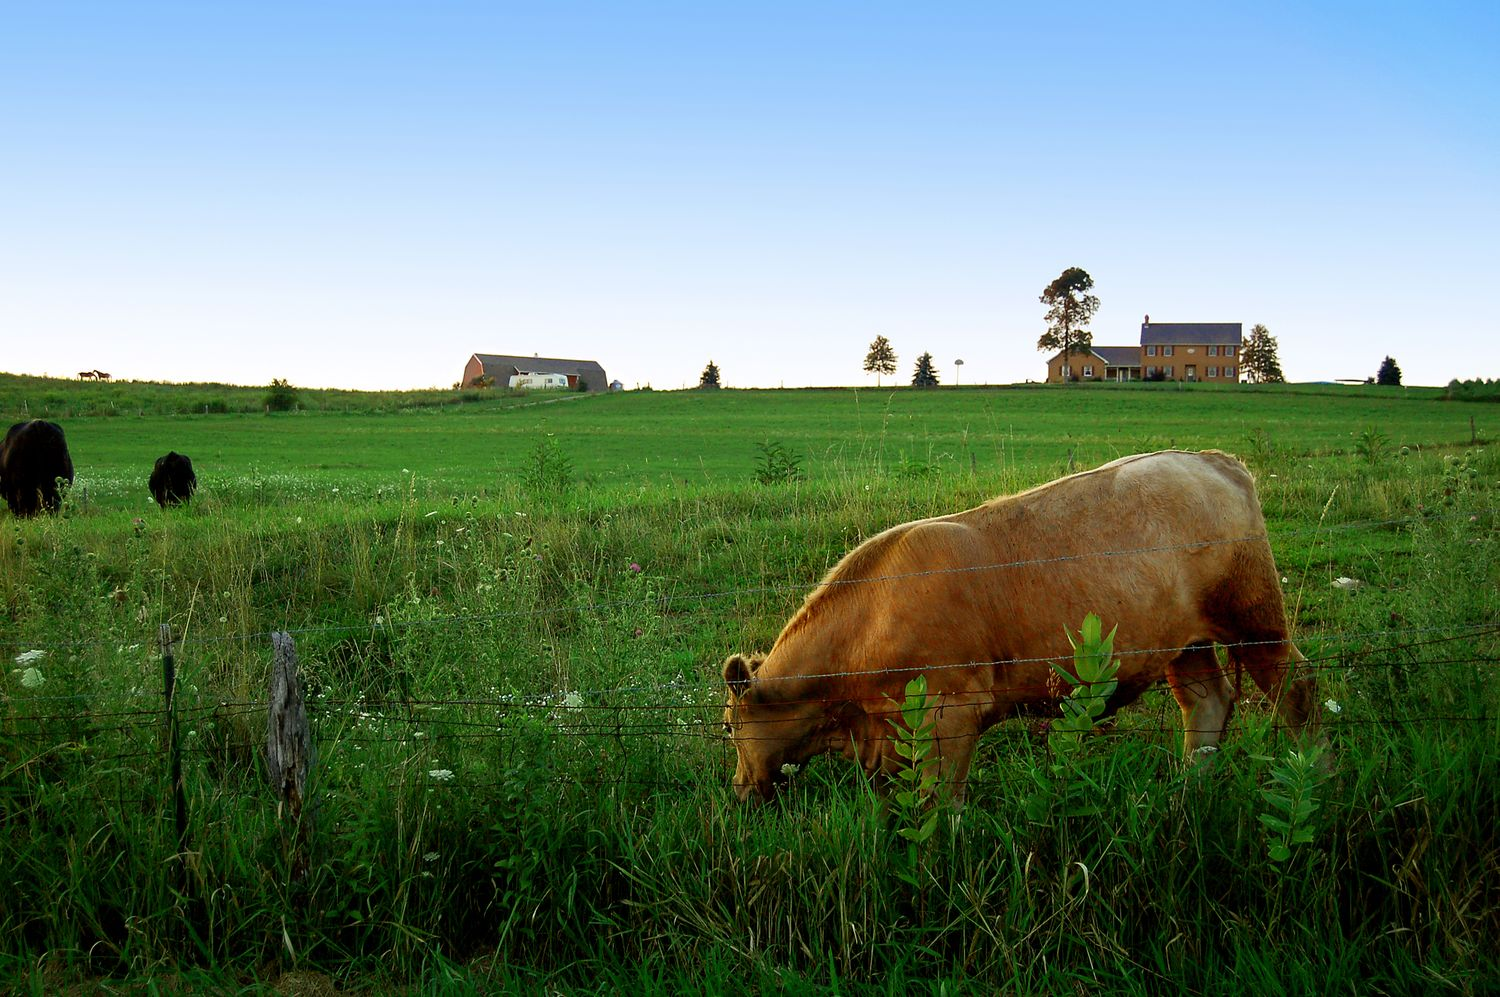
\includegraphics[scale=1]{Illustrations/Vache.jpg}
				\caption{L'élevage bovin, source de nombreuses controverses\\(Source : photo-libre.fr)}
				\label{Vache}
			\end{figure}
			
			 De plus, cette très forte concentration de bêtes dans un même espace peut poser de nombreux problèmes comme augmenter le risque d'épizootie\footnote{Une épizootie est une maladie frappant, dans une région plus ou moins vaste, une espèce animale ou un groupe d'espèces dans son ensemble. (Wikipédia)}. De telles installations servent à produire du lait en réduisant au maximum l’espace utilisé, et d’avoir une source fixe de déchets animaux afin de créer de l’énergie verte avec des méthaniseurs par exemple. De plus, du fait du nombre de vaches et donc de la production conséquente qu’une telle entrepreprise peut génerer, les grands groupes laitiers comme Agrical sont interressés. Par contre, avec de telles “usines à bovins”, si l’on étendait ce concept au territoire français dans son ensemble, le nombre d’exploitations laitières passerait de 60 000 à seulement 2500. Une telle réduction aurait forcément un fort impact social et économique en France.
			

		\subsection{L'export et la technologie de pointe, des activités porteuses}
			Malgré ce bilan plutôt négatif en ce qui concerne l’agro-alimentaire français, il reste à souligner les points positifs dans l’évolution de ces dernières années. En effet, les entreprises qui se tournent vers l’export et la technologie de pointe arrivent à garder une place importante sur le marché, voire même à se développer.
			
			La France est un pays reconnu pour ses grandes qualités d’ingénérie et d’innovation. Les exploitations françaises ont des rendements qui sont très bons et qui sont optimisés pour requérir un minimum de main d'œuvre avec un maximum d’efficacité. Ce savoir-faire s’exporte bien à l’étranger. Mais aussi, du fait de la qualité des produits français, ils s’exportent très bien. De ce fait, le secteur agro-alimentaire est le deuxième secteur le plus rentable derrière l’aéronautique avec 12 milliards d’excédants (contre 20,3 milliards pour l’aéronautique) en 2012\cite{AAExport2014}. L’exportation française croit chaque année, et en dix ans l’exportation a augmenté de 50\%. Cette progression constante est renforcée par l’idée que la France est le 5ème exportateur mondial.

	\section{La Bretagne : un cas particulier}
	Nous avons donc vu que la situation de l’industrie agro-alimentaire en France est de moins en moins bonne. Pour autant, elle semble avoir un bon ancrage dans l’économie bretonne. De manière à expliquer les caractéristiques de ce secteur en Bretagne, nous étudierons pour débuter la place de la Bretagne en France, aussi bien géographiquement qu’économiquement. Deuxièmement, nous parlerons de la place importante de l’industrie agro-alimentaire en Bretagne. Pour terminer, nous étudierons les secteurs d’activités de l’agro-alimentaire en Bretagne.
	
	% À replacer où tu souhaites, j'ai mis ça où était le commentaire sur le Drive
	
	\begin{figure}[!h]
	\centering
	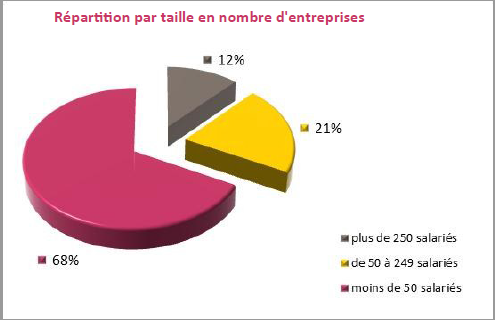
\includegraphics[scale=1]{Illustrations/RepartitionTaille.png}
	\caption{Répartition des entreprises agro-alimentaire par taille\\(Source : agro-alimentaire - Direction de l’Innovation - L’innovation dans les entreprises en 2013\cite{InnovationEntreprises2013})}
	\label{RepartitionParTaille}
	\end{figure}
	
	\begin{figure}[!h]
	\centering
	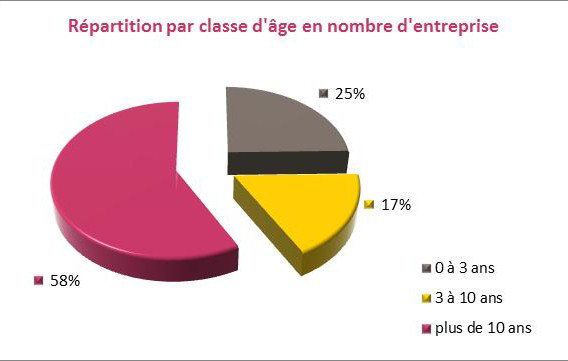
\includegraphics[scale=1]{Illustrations/RepartitionClasseAge.png}
	\caption{Répartition des entreprises agro-alimentaire par classe d'âge\\(Source : agro-alimentaire - Direction de l’Innovation - L’innovation dans les entreprises en 2013\cite{InnovationEntreprises2013})}
	\label{RepartitionParTaille}
	\end{figure}

		\subsection{La Bretagne, une exception économique et géographique}
			L’une des raisons pour lesquelles l’industrie agro-alimentaire se porte mieux en Bretagne qu’en France s’explique par la position de la région, aussi bien économiquement que géographiquement. En effet, la région présente de multiples spécificités qui font d’elle un cas à part.
			
			En effet, la Bretagne possède depuis longtemps un tissu rural très présent, de la tradition des goémoniers \footnote{Le goémonier, dénommé aussi pigoulier, est un pêcheur spécialisé dans la récolte des algues marines, plus précisément du goémon. C'est aussi le nom du bateau spécialisé utilisé pour cette récolte. (Wikipedia)} aux éleveurs de porcs, la Bretagne a, pour le reste de la France, une image campagnarde indépendante. Mais en plus de son histoire avec l’agriculture, la Bretagne s’est développée dans ce sens grâce à des spécificités géographiques. Nous pouvons voir grâce à ces cartes (Figures \ref{ReliefBathymetrie} et \ref{SAUParCommune}) la répartition de la population dans la région. Le massif armoricain étant une chaîne de montagnes de 65 000 km² culminant à un peu plus de 400m d’altitude, il a pour principal relief de vastes landes escarpées où la seule activité subsistante est l’agriculture et ses vastes pâturages d’élevage.
			
			\begin{figure}[!h]
			\centering
			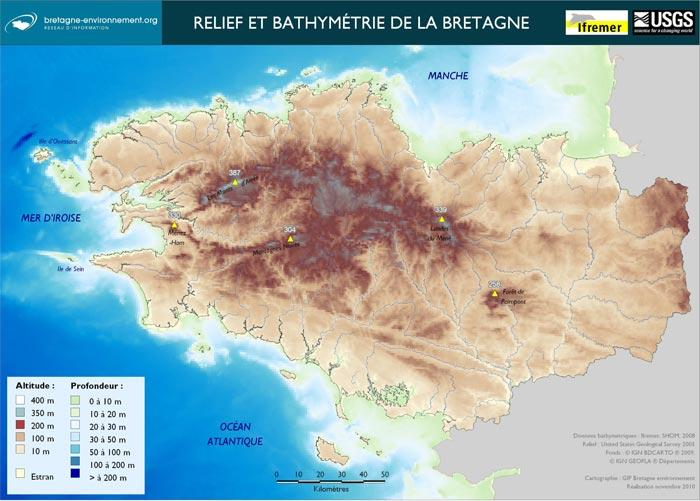
\includegraphics[width=17cm]{Illustrations/ReliefEtBathymetrie.jpg}
			\caption{Le relief de la région Bretagne\\(Source : GIP Bretagne Environnement\cite{BretagneEnvironnement})}
			\label{ReliefBathymetrie}
			\end{figure}
			
			\begin{figure}[!h]
			\centering
			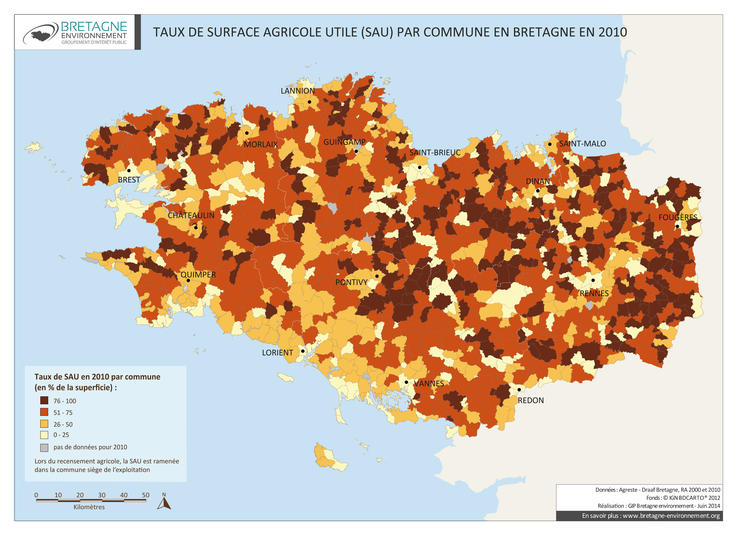
\includegraphics[width=17cm]{Illustrations/SAUParCommune.jpg}
			\caption{Le Taux de Surface Agricole Utile par commune en 2010\\(Source : GIP Bretagne Environnement\cite{BretagneEnvironnement})}
			\label{SAUParCommune}
			\end{figure}
			
			A cause de ces reliefs, nous pouvons aussi constater que la population de la Bretagne est localisée principalement proche des littoraux ou bien du bassin Rennais (Figure \ref{DensitePopulationBretagne}). Cette répartition a bouleversé le développement des littoraux bretons au niveau portuaire. Les trois principaux ports de trafic de marchandises étant Saint-Malo, Brest et Lorient qui ont réalisé en 2012 84 \% du trafic total de la région, pour un total de 8.297 millions de tonnes aux trois quarts destinés à l’Union Européenne ou au reste de la France. Ce sont également plus de 3.9 millions de passagers qui ont transité par les ports de la péninsule bretonne au cours de cette année 2012\cite{CommerceMaritimeBretagne}. On peut donc constater un développement important du commerce maritime breton qui, en majeure partie, est occupé par les produits agricoles et alimentaires (35 \%), devant les produits énergétiques (24 \%) puis la métallurgie (18 \%).
			
			\begin{figure}[!h]
			\centering
			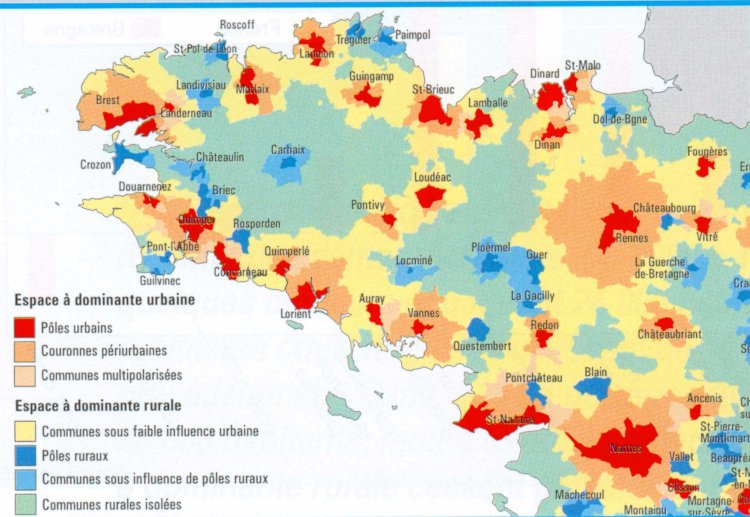
\includegraphics[scale=3.25]{Illustrations/DensitePopulationBretagne.jpg}
			\caption{La répartition de la population en Bretagne\\(Source : INSEE)}
			\label{DensitePopulationBretagne}
			\end{figure}						
			
			Mais même si la Bretagne se tourne vers l’extérieur grâce à ses échanges maritimes et que les deux tiers du trafic total de marchandises sont des échanges intra régionaux à hauteur de 120 millions de tonnes, les échanges nationaux représentent 49 millions de tonnes de marchandises donc 42\% sont des produits agricoles et alimentaires\cite{InfrastructureConnecterBretagneMondeCCI}. Ces échanges se font principalement avec les régions limitrophes de la Bretagne (90 \%). En effet, en tant que première région agricole française en termes de production, le niveau d’importation de denrées alimentaires reste limité à celles que le climat régional rend impossible à cultiver. Le fait que la Bretagne soit également la première région française au niveau de la pêche et que l’élevage soit une part importante de la production agricole, rend l’importation de ces produits une pratique très rare.
			
			Au travers de cette présentation de la Bretagne et de la place qu’occupe cette région en France, nous pouvons constater que la tendance historique d’indépendantisme breton est en partie liée à sa capacité à produire la majeure partie de ses produits de consommation en tant que première région agricole de France. Les échanges hors de la région sont principalement des exportations, par exemple en 2006, les exportations de la Bretagne représentaient 8.9 milliards d’euros contre 7.8 milliards d’euros en importation. La Bretagne occupe donc une place importante dans la production agricole française, qui était en 2012 considérée comme la 2e puissance agricole mondiale derrière les Etats-Unis.
			
		\subsection{De multiples secteurs d'activités}
			Enfin, on peut expliquer la situation de l'agro-alimentaire en Bretagne par la multiplicité des secteurs d'activités existants dans la région. En effet, non seulement cette industrie est importante dans l'économie bretonne, mais elle se présente aussi sous plusieurs formes, comme on le voit sur les graphiques ci-après (Figure \ref{SecteursIndustrielsIAA}).
			
			\begin{figure}[!h]
			\centering
			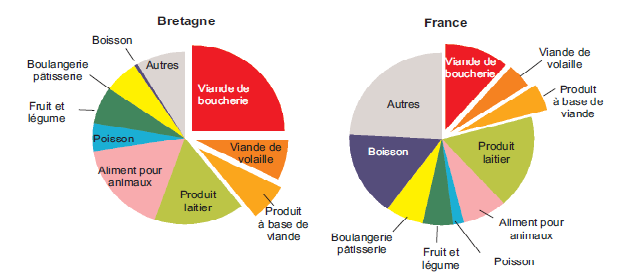
\includegraphics[scale=1]{Illustrations/SecteursIndustrielsIAA.png}
			\caption{Les secteurs industriels des entreprises de l'industrie agro-alimentaire\\(Source : INSEE - ESAN 2010 provisoire - Retraitement SSP)}
			\label{SecteursIndustrielsIAA}
			\end{figure}
			
			Si l’on regarde les chiffres de 2012, on constate qu’un peu plus de 46\% des emplois du secteur sont liés aux activités de  “Transformation et conservation de la viande et préparation de produits à base de viande”. Vient ensuite la fabrication d’aliments divers et de produits laitiers. Ces chiffres sont également liés à la taille des entreprises du secteur, en effet la majeure partie des salariés sont embauchés par des établissements de plus d’une centaine de personnes. En 2012, il y avait 4 établissements de plus de 1000 salariés :
			\begin{list}{•}{}
			\item Kermene, qui est le premier fournisseur des magasins de l’enseigne E.LECLERC en produit de boucherie et charcuterie.
			\item COOPERL ARC ATLANTIQUE, Groupe coopératif agricole majeur de la production porcine, qui est l’un des leaders bretons de la production porcine.
			\item SOCIETE VITREENE D’ABATTAGE - SVA Jean Rozé qui est spécialisée dans la conservation et la transformation de la viande de boucherie.
			\item GROUPE BIGARD qui est le leader européen au niveau de la viande bovine ainsi que le n°1 français de la viande\cite{BigardPremierTransformateurViande}
			\end{list}
			
			Tel que l’on peut le constater, les 4 plus gros établissements du secteur AA breton en 2012 étaient liés à l’élevage, à la transformation et à la conservation de la viande. Ces 4 établissements représentent 10\% des emplois du secteur et le reste des établissements les plus recruteurs sont pour la plupart reliés au secteur de la viande. Ces grosses entreprises confirment bien la tendance de la région car c’est un secteur propice à l’exportation et qui représente 57\% des ventes à l’exportation de l’IAA régionale.
			
			Les autres secteurs sont bien moins importants que celui de la viande mais la filière laitière, qui représente 10\% de l’effectif salarié du secteur de l’IAA, reste tout de meme la première de France au niveau de la production. En effet, tous les grands groupes y sont implantés tels que Lactalis, Bongrain, Danone, Entremont Alliance et bien d’autres\cite{ProduitsLaitiersRegionBretagne}. La Bretagne élève ainsi un tiers des vaches laitières françaises.
			
			Parmis les produits laitiers issus de cette activité, le produit phare de la Bretagne reste le beurre en version salée. Mais de nombreuses spécialités culinaires bretonnes telles que les crêpes, le kouign-amann, le sablé breton ou encore le caramel au beurre salé découlent de cette agriculture laitière si prononcée dans la région.
			
			La Bretagne voit également émerger des secteurs innovants dans le domaine de l’AA tels que les applications à base d’algues qui servent à diverses activités\cite{CartesBretagneagro-alimentaire20142016} : complément alimentaire, consommation directe, cosmétique, phytosanitaire ou bien pour la médecine douce.
			
			Au travers de cette étude des différents secteurs d’activité de l’industrie agro-alimentaire bretonne, bien que non exhaustive, nous pouvons constater un très fort monopole de la filière viande et laitière car ce sont des filières très sujettes à l’exportation. Certains secteurs essayent tout de même de se développer en s’appuyant sur des transformations de produits innovantes. Ceux-ci sont majoritairement portés par la production d’algues malgré le fait que l’importation d’algues étrangères reste tout de même plus compétitif que de les récolter sur place à cause du manque de structure.
			
			
	\section{La crise, impact et réponses}
		Bien que la Bretagne s’en sorte bien dans la crise de l’agro-alimentaire, cette dernière reste importante et pose de nombreux problèmes. Dans l’optique de savoir ce qui se passe autour de cette crise, nous commencerons par comparer ses impacts au niveau national et au niveau breton. Nous verrons ensuite quelles sont les actions menées par les pouvoirs publics. Enfin, nous parlerons des solutions envisagées pour l’avenir.
		
		\subsection{La Bretagne en meilleure posture que le France}
			\paragraph{}Avant de pouvoir parler de la réaction générale face à la crise, regardons pour commencer ses impacts. Afin de mieux nous rendre compte de la différence des conséquences en France et en Bretagne, nous procéderons tout d'abord à une analyse de l'impact aux différentes échelles, puis nous comparerons les résultats.

			\paragraph{}Dans un premier temps, intéressons-nous à ce que représente la crise au niveau national. En raison de l'importance que l'industrie agro-alimentaire a dans le pays, il paraît normal de penser que le secteur ait subi la crise de plein fouet, au moins sous certaines formes. La première des conséquences de la crise dans l'agro-alimentaire français est une conséquence de centralisation\footnote{La centralisation dans le domaine économique désigne l'action consistant à grouper des activités le long de la chaîne de production dans une seule entreprise.}. En effet, les petites organisations résistent moins bien face à de tels évènements, poussant ainsi les plus grosses structures à effectuer des rachats ou à améliorer leur solidité. Par exemple, le groupe Intermarché a effectué le rachat des abattoirs Gad en Octobre 2014 pour les intégrer à sa filiale SVA Jean Rozé. Ces mêmes rachats ont pour but, entre autres, de diversifier leurs activités pour conforter une place qui tend à se fragiliser. En outre, avec les baisses des aides de la Politique Agricole Commune (pour l’exemple, l’Union Européenne a diminué de 24,5\% les subventions européennes et de 45,4\% les subventions nationales), les ressources financières du secteur se raréfient dangereusement, mettant en péril certaines branches de l’industrie. On peut citer, à titre d’exemple, la filière de la volaille, dont plusieurs représentants, à l’instar de Doux se retrouvent au bord de la fermeture. Cela provoque également une augmentation de l’importation, puisque le solde entre production et consommation diminue de plus en plus et de plus en plus vite (-22\% de 1996 à 2000 puis -40\% de 2000 à 2005)\cite{AvenirExploitationVolailleBretonne}.

			Qui plus est, la crise se manifeste aussi par une crise de confiance. Effectivement, outre la “vache folle de 1986 à 1996”, de multiples scandales se sont accumulés dans l’agro-alimentaire sur la dernière décennie\cite{Scandales} : la grippe aviaire en 2006, les problèmes sur les produits importés la même année, le lait à la mélamine en 2008, l’Escherichia Coli dans les concombres en 2011, les steaks hachés contaminés en 2012, la fraude à la viande de cheval en 2013. À cause de cela, les modes de consommations changent. Plus précisément, les consommateurs se tournent vers les commerces de proximité, car les différents scandales sont majoritairement nés de l’import en masse des grands groupes industriels.
			
			\begin{figure}[!h]
			\centering
			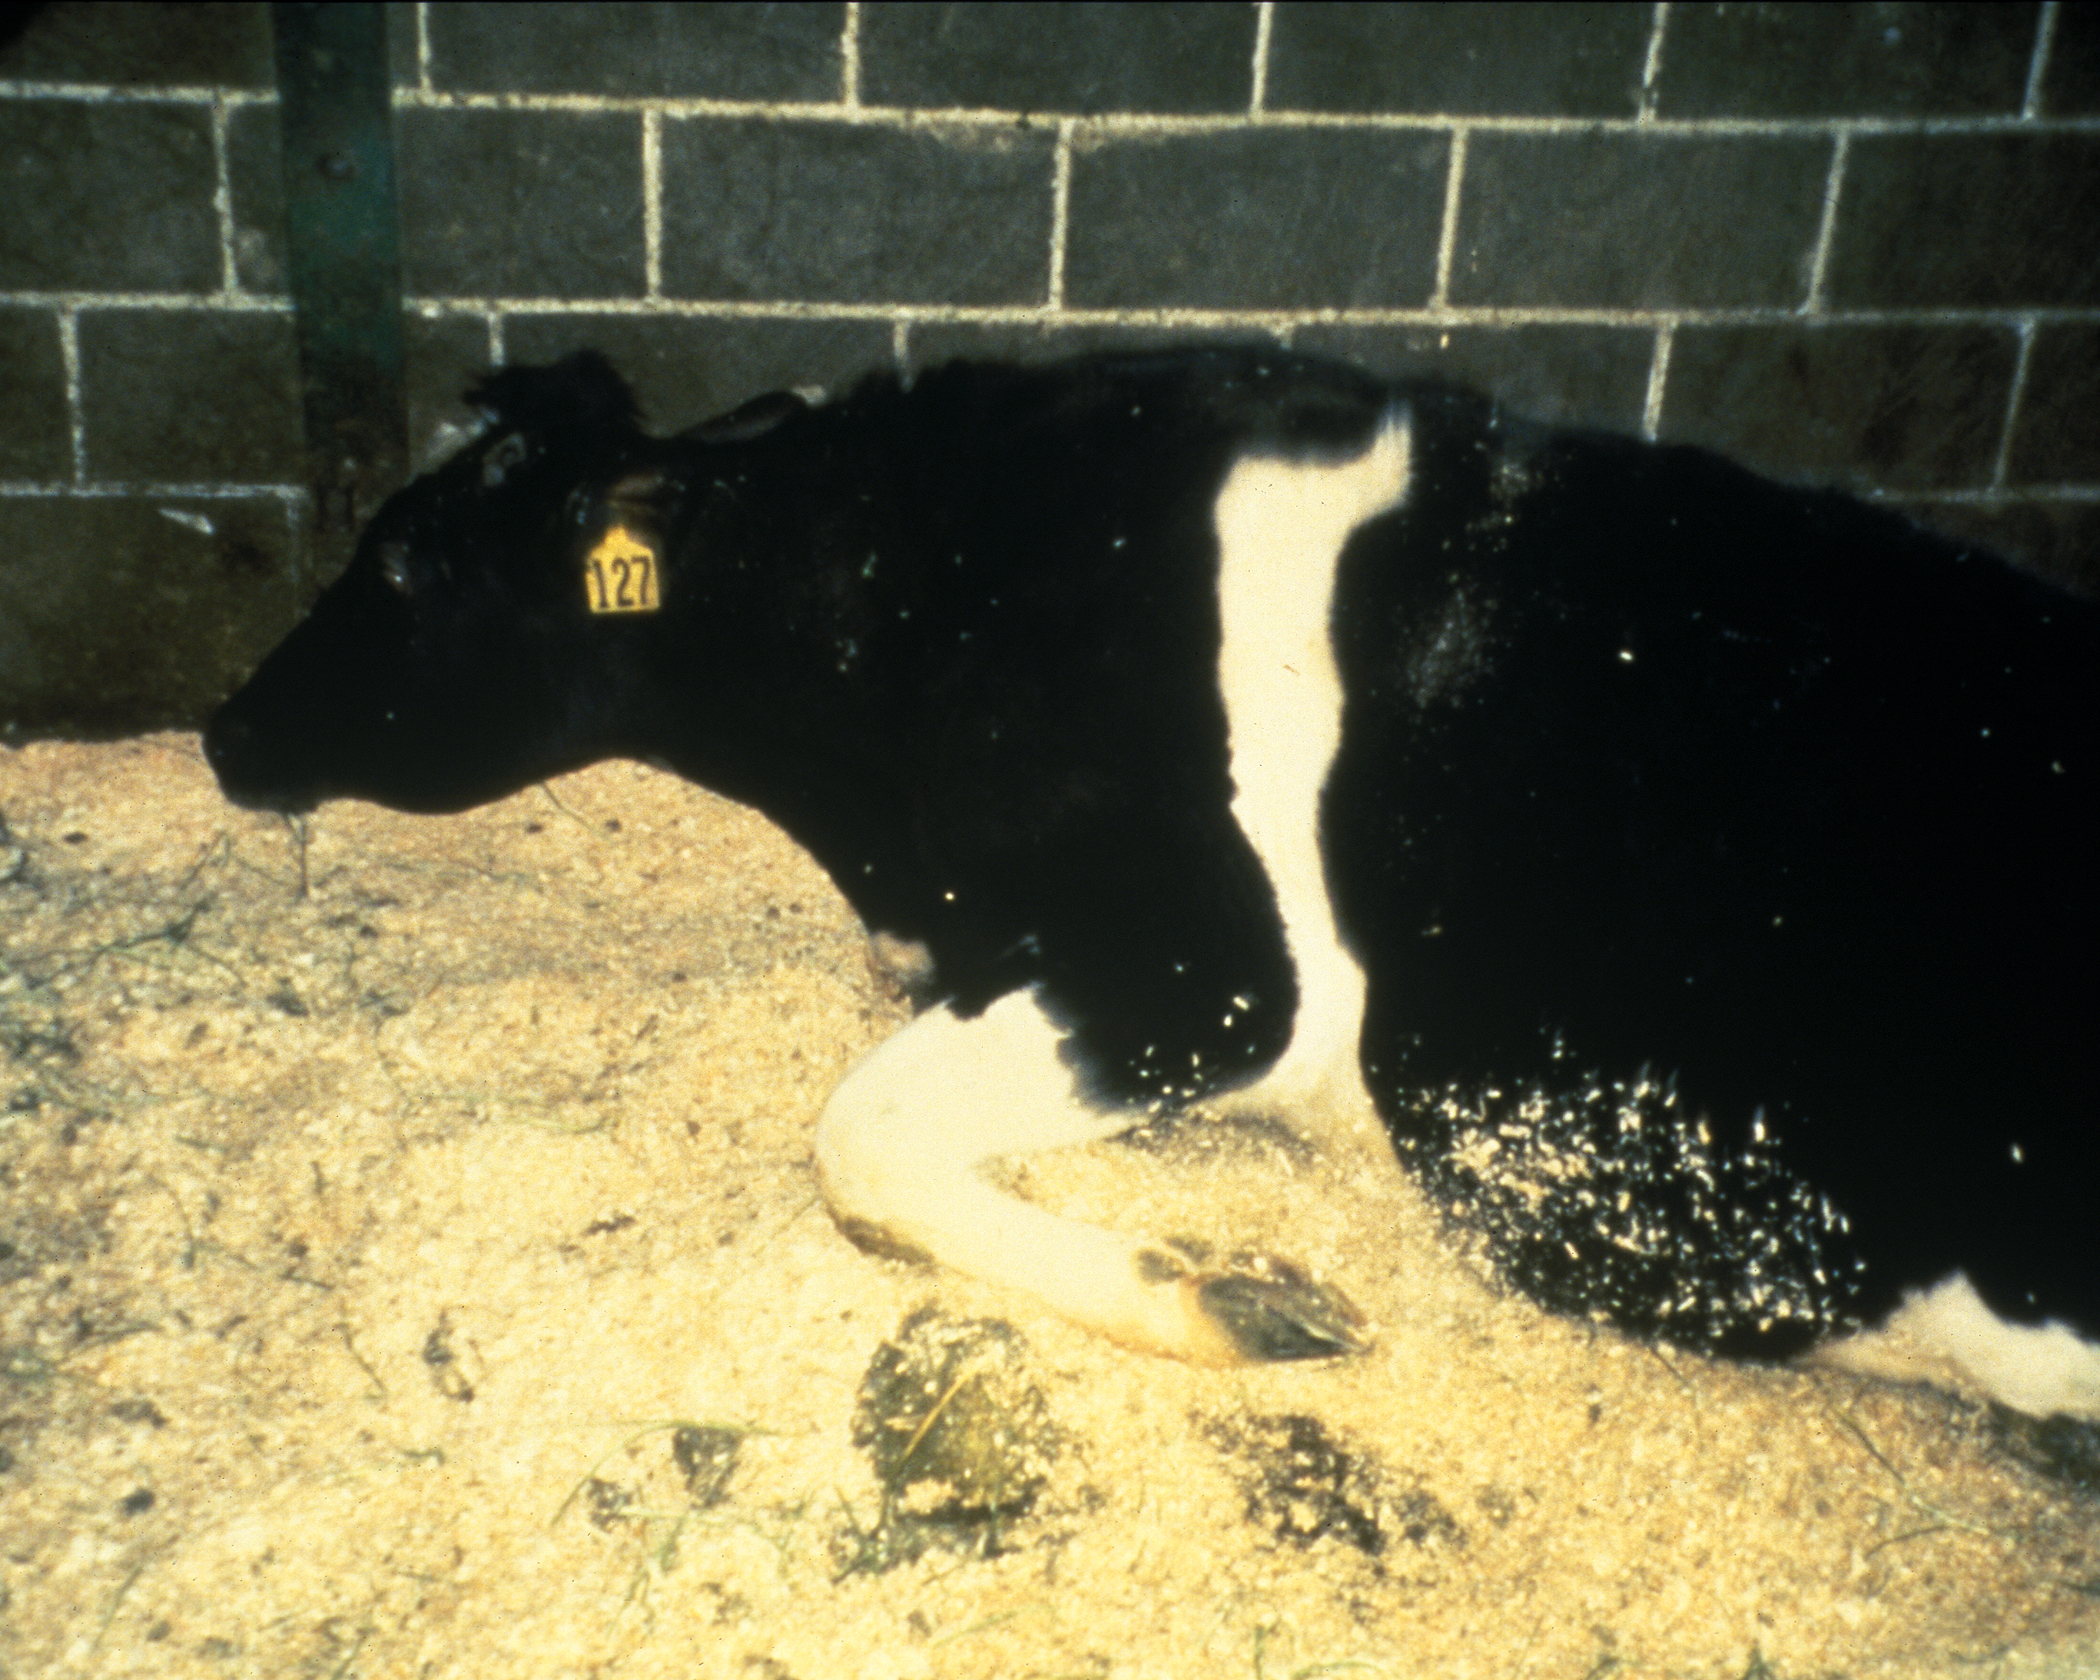
\includegraphics[scale=0.5]{Illustrations/VacheFolle.jpg}
			\caption{La crise de la vache folle, un choc important pour toute la filière bovine\\(Source : Wikipedia)}
			\label{VacheFolle}
			\end{figure}
			
			D’un autre côté, des spécificités se présentent à l’échelle régionale. En Bretagne, l’agro-alimentaire est une industrie relativement importante pour l’économie, mais c’est surtout une force majeure pour la région, comme nous l'avons décrit précédemment. Ainsi, on voit que même si certaines organisations sont en difficulté, la présence de l’agro-alimentaire à différents niveaux permet de se passer du recours à des intermédiaires étrangers. Ce fait met donc en évidence l’existence d’une synergie entre les acteurs de la région.

			De ce fait, nous pouvons mettre en opposition deux situations : celle de la Bretagne et celle de la France. Ainsi, on voit que le secteur se retrouve dans une position difficile au niveau de la France, en raison de l’existence de marchés étrangers plus compétitifs et donc plus avantageux que les marchés locaux pour les distributeurs, mais aussi à cause du manque de confiance croissant des consommateurs. Mais l’état des choses en Bretagne est tout autre, puisque la région reste ancrée dans cette industrie, comme il a été précisé plus tôt, et que le soin que la région y porte lui offre un délai permettant de trouver des réponses plus efficaces et donc de faire plus aisément face à la crise.

			\paragraph{}Ainsi, nous pouvons sans trop de problèmes affirmer que la Bretagne est dans une meilleure situation que la France
			
		\subsection{Différentes actions à différentes échelles}
			\paragraph{}En réponse à cette crise, les pouvoirs publics ont mis en œuvre de nombreuses actions, plus ou moins efficaces. Mais ces actions ne sont pas toutes venues du même échelon. En effet, certaines d'entre elles ont été menées au niveau national, d'autre à des niveaux plus locaux. Afin de mieux nous en rendre compte, nous commencerons par voir les actions du gouvernement. Ensuite nous verrons ce qui a été fait par la région et les départements.

			\paragraph{}Tout d’abord, le gouvernement a apporté des mesures dans le but de répondre aux problèmes de l’industrie agro-alimentaire. Pour commencer, le gouvernement a décidé en décembre 2013 de mettre en place le Plan Agricole et agro-alimentaire pour l’Avenir de la Bretagne au sein du Pacte d’Avenir\cite{PacteAvenirBretagne}. Cette action vise à apporter à la Bretagne des solutions à la fois pour pallier au déficit d’emplois de ces dernières années, mais aussi à soutenir les entreprises en difficulté. Pour ce faire, des subventions sont prévues pour les entreprises en difficulté, ce qui permet à la fois d’éviter les licenciements et d’aider les entreprises à se redresser. En outre, ce programme cherche à accorder plus d’importance au renouvellement des activités, par l’intermédiaire de l’innovation par exemple. De manière justement à mettre l’accent sur ce point, un soin tout particulier a été accordé aux pôles de compétitivité et aux instituts de recherche. Ainsi, l'une des initiatives prises est la mise en place de l’institut Carnot pour aider les entreprises à vérifier l’état des choses dans leur activité. L’importance donnée aux pôles de compétitivité vise quant à elle à rendre les entreprises capables d’améliorer et d’élargir leurs gammes de produits en fonction de ce qui est en vogue.

			Pour répondre aux questions que se posent les consommateurs sur la qualité des produits qu’ils achètent, une autre mesure a été votée le 11 Février 2014 pour promouvoir la viande d’origine française au travers de sept logos, selon le type de viande en question (voir Figure \ref{VDF}). Cette décision fait suite à la crise de la fraude à la viande de cheval et a pour but de permettre au consommateur de savoir d’où vient ce qu’il mange et d’être ainsi plus sûr de la qualité du produit. Néanmoins, avec le nombre important d’importations pour tout ce qui est animal, l’apparition de ce logo reste encore très rare. En Septembre, un constat a été fait sur les étals. Mis à part pour la volaille où 55\% des produits mis en rayon affichent le logo, les chiffres sont catastrophiques. Seulement un peu plus de 2\% des produits à base de porc affichent ce logo, ce qui prouve le peu d’importance donnée à l’origine de la viande par les entreprises\cite{FlopVDF}.

			\begin{figure}[!h]
			\centering
			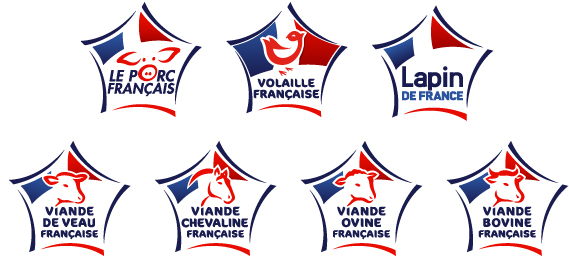
\includegraphics[scale=0.5]{Illustrations/VDF.jpg}
			\caption{Les logos Viande de France}
			\label{VDF}
			\end{figure}

			Une autre des mesures prises l’est par la région. En effet, même si le conseil régional a participé à la création du Plan cité précédemment, des décisions se voulant à la fois plus précise et plus en accord avec la situation régionale ont été faites. La politique régionale, depuis le début de l’année 2014, est d’améliorer la qualité des produits proposés par l’industrie agro-alimentaire\cite{FavoriserQualiteAgricultureagro-alimentaire}. Pour cela, l’accent est mis sur le respect de l’environnement et la production d’énergies propres. Nous pouvons constater que cela fait suite aux crises de l’agro-alimentaire qui ont provoqué la perte de confiance des consommateurs. Ainsi, en produisant mieux plutôt que plus, la région compte répondre aux attentes de la société actuelle en matière de consommation.

			Enfin, les entreprises elles-mêmes cherchent à prendre des mesures pour sauver leur activité. Nous pouvons, pour cela, citer une seconde fois le rachat des abattoirs Gad par Intermarché. Cette action se motive non seulement par des choix économiques dans le groupe, mais également par la volonté de fortifier la SVA Jean Rozé dans son activité d’exploitation de viande animale. Ainsi, en effectuant ce que l’on appelle l’intégration verticale, qui est pour une entreprise l’extension de ses activités le long de sa filière, le groupe se détache d’intermédiaires coûteux et présentant des risques pour sa pérennité. En outre, en étendant son activité, la filiale peut se pencher sur la question d’une modification de la gestion de son activité, et se moins se focaliser sur son cœur de métier tout en déplaçant des ressources sur la recherche et le développement de produits innovants.

			\paragraph{}En conclusion, des actions différentes ont été mises en place à plusieurs niveaux, mais il est important de noter que ces actions rejoignent majoritairement le même but : innover pour plaire au consommateur.

			
		\subsection{Quelles solutions pour l'avenir ?}
			Suite aux problèmes qui se posent aujourd'hui dans l’agro-alimentaire, il est important de se rendre compte des solutions envisagées pour l’avenir de cette industrie. Pour voir cela, nous commencerons par voir quelles sont les solutions envisagées par les entreprises. Ensuite, nous nous intéresserons à ce que prévoit l’État pour les prochaines années.
			
			Pour débuter, voyons quelles actions les entreprises considèrent pour les prochaines années. Pour beaucoup d’entreprises, la solution se trouve dans l’intégration verticale. Ainsi, de nombreux groupes étendent leur activité pour avoir un meilleur contrôle sur la filière. Pour autant, cette solution n’est l’apanage que de grandes structures. Par conséquent, les plus modestes entreprises se tournent vers un autre moyen de faire face : l’innovation. On constate aujourd’hui que le nombre d’entreprises dans le secteur de l’agro-alimentaire se répartit de manière peu équitable. En effet, en 2008, plus de 90\% de ces entreprises étaient des PME\cite{IAAFranceChiffres}. Cela montre ainsi que ce n’est pas forcément l’importance de l’organisation qui lui permet de perdurer dans cette industrie, mais plutôt son activité. C’est pour cette raison qu’un nombre sans cesse plus important d’entreprise tente de restructurer son activité afin de moderniser leur image et de renouveler l’intérêt que les consommateurs peuvent leur porter. Un autre constat est la dispersion des entreprise sur un plan géographique. Non seulement beaucoup d’entreprises sont éloignées les unes des autres, mais en plus elles ne cherchent que peu la collaboration. C’est pourquoi les plus importantes organisations veulent créer dans les prochaines années une synergie qui paraît être la clé pour la solution à de nombreux problèmes.
			
			\begin{figure}[!h]
			\centering
			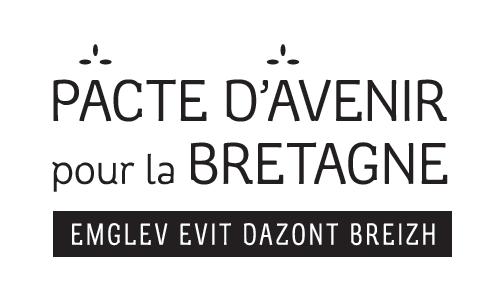
\includegraphics[scale=1]{Illustrations/Pacte_Avenir_Bretagne.png}
			\caption{Le Pacte d'Avenir pour la Bretagne, une solution efficace ?}
			\label{PacteAvenirPourBretagne}			
			\end{figure}
			
			Ensuite, Le gouvernement prévoit lui aussi des actions. Dans ses prochains plans économiques, il compte continuer sur la même voie afin de solidifier ce qui est d’ores et déjà en place. Ainsi, on peut se rendre compte que le Plan Agricole et agro-alimentaire pour l’Avenir de la Bretagne au sein du Pacte d’Avenir précité prévoit des réponses sur le court voire moyen terme, plus précisément pour l’horizon 2020 au maximum. Mais que prévoient les pouvoirs publics pour après cette date ? Le ministère de l’agriculture a décidé de mettre en avant trois grands points sont au goût du jour pour 2025\cite{AvenirFiliereAgricole2025}. Le premier d’entre eux est la réponse aux aléas. En effet, avec la multiplication des catastrophes naturelles ces dernières années (et en particulier l’année 2014). Un autre de ces aléas est un aléa plus financier : de plus en plus, les prix dans l’agro-alimentaire sont sujets à la volatilité, en raison des spéculations fortes sur ce secteur. Sur un domaine plus proche de l’industrie, l’État compte renforcer la coopération entre les entreprises, au moyen de simplification des démarches pour celles qui le souhaitent. De ce fait, une synergie peut se mettre en place et donc provoquer une amélioration pour chaque acteur. Pour terminer, le dernier point pensé par le ministère est la formalisation de stratégies commerciales pour développer plus efficacement les échanges entre entreprises et la communication entre entreprises et consommateurs. Ces mêmes stratégies commerciales se veulent également moyen de consolider les marchés d’exportation, qui représente l’une des activités qui se portent le mieux pour l’industrie agro-alimentaire.
			
			Pour conclure, on voit qu’il existe des solutions de différents ordres pensés pour faire face à la crise dans les prochaines années. Certaines correspondent à la vision qu’à chaque entreprise de son activité, tandis que d’autres partent de la situation économique actuelle au niveau national.
			
\chapter{L'innovation, un remède contre la crise}
	
	\section{Les différentes formes d'innovation}
	
		\subsection{De nouveaux modes de production}
			L’agriculture bretonne s’est petit à petit intensifiée, en effet, depuis les années 70, les travaux se sont de plus en plus mécanisés, les machines sont devenues quasiment omniprésentes dans l’agriculture de nos jours. De plus, par le développement de la recherche sur l’agriculture, de nouveaux outils sont apparus pour permettre “l’augmentation de la productivité et une meilleure sécurité alimentaire”\cite{FAOStatisticalYearbook2013}. Parmi ces outils, on peut citer le GPS dans un tracteur moderne\cite{RobotsChamps} qui permet d’optimiser un circuit dans le cadre de répartition d’engrais.
			
			\begin{figure}[!h]
			\centering
			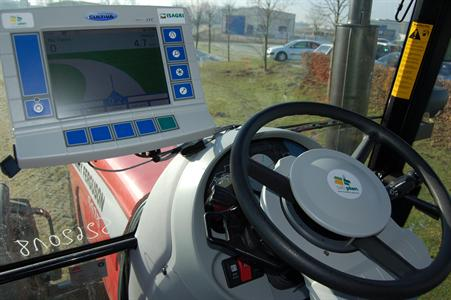
\includegraphics[width = 200 pt]{Illustrations/GPS_Tracteur.jpg}
			\caption{Le GPS, un outil important pour l'agriculture de demain\\(Source : terre-net.fr\cite{GPSEtTracteur})}
			\label{GPSTracteur}
			\end{figure}
			
			L’utilisation de machines, d’engrais et d’arrosoirs automatisés permet un meilleur rendement qu’une pousse naturelle, c’est-à-dire sans intervention de l’homme après ensemencement. On en vient à parler de mécanisation des champs, ce qui facilite le travail pour l’agriculteur, dans un monde où les parcelles s’agrandissent et où la demande de nourriture est de plus en plus importante.
			
			Du côté de l’élevage, on note la recherche sur le bon développement des animaux, sur le développement de l’élevage en batteries et, entre autres, le rationnement en oligo-éléments\cite{OligoElements}. Effectivement, les bovins, porcins et autres animaux d’élevage ont besoin d’un apport en différents minéraux. Cette affirmation en elle-même est le résultat d’études sur le métabolisme de ces animaux, ce qui débouche sur un contrôle de l’alimentation plus précis et une amélioration de la sécurité alimentaire.
			
			Evidemment, toute cette émulation autour de l’agriculture a aussi permis de développer d’autres modes de production peut-être moins éreintant pour le sol et les animaux comme la rotation des cultures qui permet de préserver la fertilité des sols et de diversifier la production.
			
			\begin{figure}[!h]
			\centering
			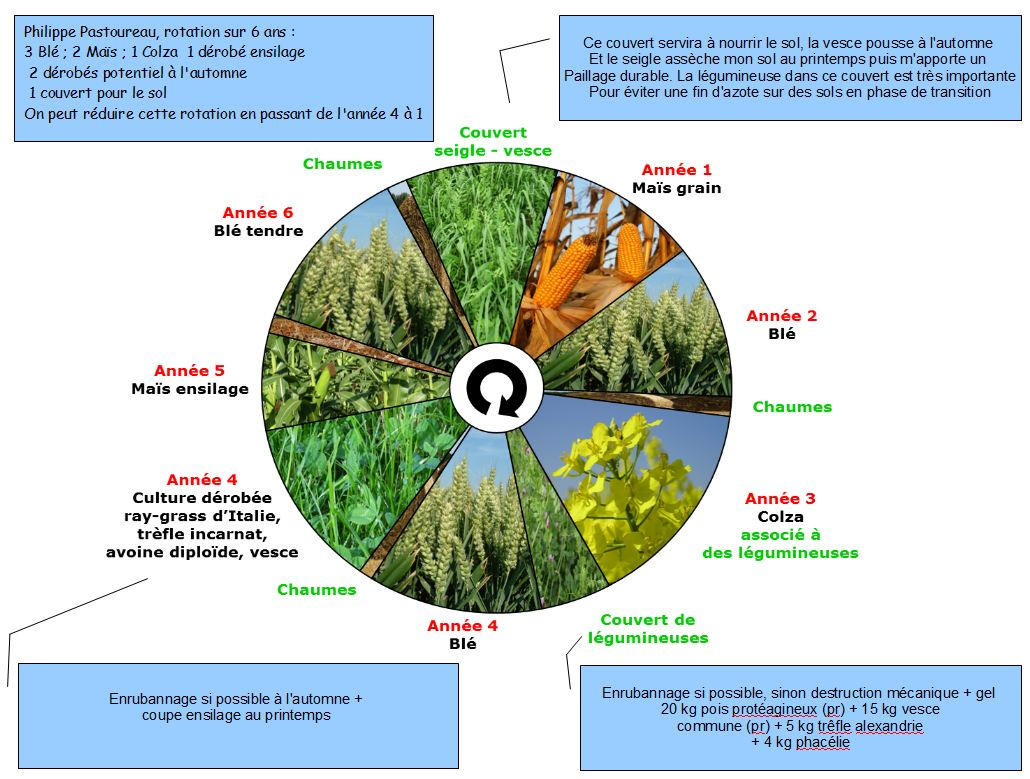
\includegraphics[scale=0.6]{Illustrations/Rotation.jpg}
			\caption{\\(Source : agriculture-de-conservation.com\cite{RotationSite})}
			\label{Rotation}
			\end{figure}
			
			Au sein même d’une entreprise on peut aussi explorer différentes pistes d'innovation. Nous pouvons prendre l’exemple de Nespresso qui innove par son service et par sa communication dans le monde du café afin d’en faire un produit de prestige aux yeux des consommateurs.
			
			Prenons maintenant Valorial comme exemple: Ils s'intéressent surtout aux projets autour d'une vrai innovation concrète en Recherche et Développement et à vocation industrielle et compétitive, donc au niveau du développement du produit. Toutefois, récemment, ils ont accepté des projets liés au marketing. Mais il est difficile de trouver une communication innovante sur l'agriculture, à l'image des multitudes de publicités exhibant des procédés écologiques, respectueux des animaux, des Hommes et de l'environnement. 
			
			Il est important de souligner que les innovations ne se répercutent pas instantanément sur l'exploitation, nous exposerons plus loin dans la monographie cette inertie. De même nous découvrirons les critiques portant sur le développement des nouvelles technologies, mais nous devons garder en mémoire qu’il est nécessaire d’évoluer pour rester compétitif.
			
			
		\subsection{L'organisation des entreprises repensée}
			Au cours du temps, de nouvelles structures d’organisation, que l’on doit aussi appeler innovations, apparaissent.
			
			Comme dit plus haut dans les solutions envisagées en temps de crise, les petites et moyennes entreprises en temps de crise peuvent se regrouper en collectivités et en coopératives pour résister aux crises : c’est aussi une forme d’innovation, que l’on peut qualifier de socio-économique, qui permet à plusieurs petits producteurs ou industriels de se faire entendre et peut-être d’innover ensemble. 
			Mais cette collaboration n’est pas réservée aux structures modestes,mais à toute organisation ou entreprise qui souhaite évoluer dans un groupe. Nous pouvons constater par exemple, de grandes entreprises parmi les partenaires du pôle de compétitivité Valorial comme l’Ifremer.
			
			Evidemment, l’absorption de petites entreprises par une, plus grande, est aussi une forme d’innovation socio-économique. En effet, cette intégration permet tout d’abord à la petite entreprise de revoir son mode de fonctionnement global et surtout de revoir ses priorités en terme de communication b2b (business to business). La petite entreprise devra donc à l’avenir travailler en collaboration avec une partie ou toutes les sous-structures de la grande enseigne.
			Du côté de l’entreprise intégratrice, on peut aussi affirmer que des modifications au sein de la gestion de l’entreprise devront se faire pour que la petite entreprise soit bien intégrée. 
			
			
				
		\subsection{L'utilisation de nouvelles ressources}
			Nous allons maintenant examiner le cas de l’exploitation des algues en Bretagne.
			Avant tout il faut préciser que toutes les espèces d’algues ne sont pas utilisées. Parmi celles qui le sont, on remarque que certaines sont préférées dans un domaine d’application ou dans un autre. Dans notre exemple nous nous focaliserons sur le domaine de la cosmétique et nous ferons un constat de différents types d’innovations qui ont permis cette exploitation.
			
			Tout d’abord, intéressons-nous aux innovations scientifiques. En effet, c’est parce que les techniques en laboratoire se sont développées que les vertus des algues peuvent être extraites et utilisées. On parle de principes actifs, de protéines, de vitamines et d’autres produits bénéfiques pour le corps humain que l’on retrouve dans le végétal.
			
			Dans un deuxième temps, nous devons expliciter les types de structures au sein d’une entreprise qui se développent pour pouvoir utiliser les algues. Nous trouvons donc des chaînes de production, de la culture dans des lieux spécifiques (île d’Houat pour Daniel Jouvance)\cite{Algues}, un développement de la communication envers les clients et peut-être même de nouvelles relations entre les entreprises.
			
			Nous pouvons remarquer dans la base de données de Valorial que les algues sont surtout utilisées en complément alimentaire pour le bon développement des animaux ou dans la fabrication de plats. On remarque tout de même un projet qui utiliserai les algues pour protéger des cultures. Peut-être serait-il possible d’élargir le champs d’application des algues, mais toujours dans le domaine de l’agro-alimentaire. 
			
			Il serait intéressant de poursuivre les efforts dans l’utilisation des algues, notamment concernant l’algue verte en Bretagne qui est actuellement un fléau mais qui, peut-être pourrait devenir un avantage pour la région si un projet durable aboutit. 
			
	\section{Comment fait-on pour innover ?}
			
		\subsection{La recherche au sein des entreprises}
			Un projet d’innovation commence par une idée qui peut apparaître pour différentes raisons. La plus commune est la mise en évidence d’un besoin qui déclenche la recherche d’une solution. Par exemple le plan Ecophyto\cite{RobotsChamps} qui a pour but de limiter l’utilisation de désherbant chimique pourrait provoquer l’apparition de projets de machines de désherbage automatisés. 
			Des découvertes scientifiques peuvent également ouvrir de nouveaux marchés et de nouvelles possibilités pour les entreprises. 
			
			On peut par exemple citer Bellegum\cite{Bellegum} qui a pu, grâce à Valorial, lancer une gamme innovante de mousse aux légumes. Grâce à ces produits, l’entreprise a pu se hisser au niveau mondial, en voyant le groupe Intermarché proposer ses produits en rayon depuis début 2013.
			Enfin les interactions et la coopération avec les différents acteurs permettent aux entreprises de faire des innovations organisationnelles.
			
			Pour démarrer et aller au bout d’un processus de recherche, il ne suffit pas d’avoir une idée mais il faut également trouver les ressources la mener à bien.
			
			L’innovation dans le milieu industriel est avant tout issu de l’apprentissage des entreprises. Cet apprentissage est directement lié à la capacité de l’entreprise à gérer l’expérience qu’elle produit. En effet, par l’usage de nouvelles technologies elle en perfectionne la maîtrise ce qui conduit a une plus grande acceptation de la part des utilisateurs et donc une amélioration du produit. 
			L’apprentissage de l’entreprise est également dépendant de sa capacité à interagir avec les autres acteurs, en particulier ses fournisseurs et ses clients, afin de travailler ensemble dans l’adaptation aux nouvelles technologies.
			
			C’est cet apprentissage qui conduit l’entreprise à développer une base de connaissance qui servira tout au long du processus de recherche et d’innovation.
			
		\subsection{Les acteurs à prendre en compte}
			Les idées novatrices peuvent apparaître partout, et si les grosses entreprises ont les moyens d’investir dans de la recherche et du développement, ce n’est pas le cas des PME. C’est pourquoi les pôles de compétitivité, tel que Valorial, ont un rôle très important dans le processus d’innovation. Ils commencent tout d’abord par sélectionner les projets sur certains critères. Le Pôle Valorial spécifie dans ses critères d’éligibilité\cite{Eligibilite} qu’un projet pour être valide doit être dans une des thématiques du pôle, à savoir : “Technologies innovantes / Sécurité alimentaire / Nutrition santé animale ou humaine / Ingrédients fonctionnels”, qu’il doit être collaboratif, c’est à dire bénéficier de partenaires industriels et académiques, et qu’il doit être “source de création de valeur et de croissance pour les partenaires”.
			
			Une fois un projet sélectionné, le pôle de compétitivité accompagne l’entreprise dans le processus de recherche et de développement, et la conseil dans les démarches à réaliser. En particulier le pôle de compétitivité permet de trouver des financements via différents fonds : majoritairement l’État mais également la région / le département, les fonds d’investissement, les banques…
			A travers le pôle de compétitivité, l’entreprise peut trouver les compétences nécessaires à la réalisation de son projet.
				
		\subsection{La mise en place du produit}
		Les conséquences de l’innovation dans le secteur de l’agro-alimentaire sont nombreuses. On remarque un regain d’intérêt de la part des consommateurs pour une agriculture bretonne jugée essentielle au développement régional. De fait, 78\% des personnes interrogées lors du sondage de Agriculteurs de Bretagne pensent que l’agriculture crée directement ou indirectement de l’emploi en Bretagne et 94\% pensent que l’agriculture est indispensable au développement de la région\cite{AgriculteursDeBretagne}. De plus, les consommateurs considèrent les produits bretons comme des produits de qualité et ont remarqué les efforts des industriels pour respecter l’environnement avec pour conséquences un impact positif sur le marché de l’agro-alimentaire.

    Au delà de la vision du grand public, l’innovation est largement au service des entreprises. Elle permet aux petites entreprises de se faire une place en se démarquant grâce à des produits innovant. En effet le profit ne se situe pas toujours dans la vente en masse mais dans la vente de produits ciblés qui répondent à un besoin encore inassouvi ou qui parfois créent même le besoin et la réponse. Ce mode de fonctionnement permet à de petites ou moyennes enreprises de se hisser sur le marché mondial.
Les grandes entreprises s’intéressent également à l’innovation pour améliorer leur organisation, leurs processus de production et leurs stratégies de marketing.
Certaines entreprises se développent complètement sur le principe de l’innovation, pas en créant de nouveaux produits ou de nouveaux processus mais en mettant en relation entreprises, centres de recherche et financeurs pour mener à bien leurs projets, comme le pôle de compétitivité Valorial.

	L’innovation offre également la possibilité de passer sur des secteurs plus porteurs pour certaines entreprises dont l’activité s'essouffle. On peut remarquer le développement de nouveaux secteurs dans le domaine de l’agro-alimentaire, comme la nutrition médicale.
			
	\section{Une structure pour l'innovation : le pôle Valorial}
		
		\subsection{Une structure orientée vers l'innovation}
			Valorial est le pôle de compétitivité (c’est-à-dire un rassemblement d’entreprises et d’établissements de la recherche) au coeur du 1er bassin agro-alimentaire d’Europe\cite{SiteValorial}, en effet la Bretagne est non seulement la première région agricole et agro-alimentaire française, mais également la première région exportatrice d’Europe en agro-alimentaire\cite{RennesAtalante} ! Fondé en 2006, le pôle Valorial s’étend aujourd’hui jusqu’aux Pays de la Loire et en Basse-Normandie.


			 Fort de ses 270 membres (industriels, centres de recherche et établissements d’enseignement supérieur), le coeur de métier du pôle Valorial est d’accompagner les projets en soumettant les idées innovantes à des entreprises, en recherchant des partenaires pour la R \& D et les financements mais également en apportant une ingénierie financière et une vision aguerrie sur le projet. 
			
			 Il existe de nombreux pôles de compétitivité, et chacun à sa propre manière de fonctionner. Chez Valorial, le déroulement d’un projet se découpe en plusieurs étapes. L’idée peut provenir directement d’industriels à la recherche de moyens, ou bien être émise par Valorial lui-même. Le projet doit ensuite être validé et passe devant un consortium d’une douzaine de personnes extérieures qui représentent des structures telles que la Chambre de Commerce, la technopole de Rennes Atalante, l’Institut National de la Recherche Agronomique afin d’être labellisé. Valorial peut alors présenter le projet devant les financeurs potentiels. (Annexe \ref{Interview})

			L’objectif de Valorial n’est pas d’apporter un soutien d’ordre technique mais bien de mettre en relation les différents acteurs. Toute entreprise ou laboratoire ayant des compétences de R \& D dans le domaine du projet est susceptible de devenir partenaire. Une grosse partie du travail consiste à trouver des fonds. Pour cela il y a plusieurs sources, certaines du publique et d’autres du privé. Dans le domaine publique, les principaux financeurs sont les collectivités territoriales (Bretagne, Pays de la Loire, Basse-Normandie) mais pour certains projets et il est également possible de recourir au Fond Unique Interministériel (FUI), en particulier lorsque les collectivités territoriales ne peuvent pas aider les partenaires car ils se trouvent hors du territoire national. (Annexe \ref{Interview})

			Les fonds du domaine publique représentent environ 60\% du financement, le reste étant des fonds privés qui proviennent des cotisations des adhérents. En effet chaque adhérent au pôle Valorial paie une cotisation pour avoir accès aux différents services tels que la labellisation de projet, les invitations aux salons, etc. Cette cotisation est proportionnelle à la taille de la structure.  (Annexe \ref{Interview})
    
    			Cependant le pôle Valorial ne s’intéresse pas tous les projets. Ces derniers doivent satisfaire à certains critères d'éligibilité, et en particulier le projet doit être innovant dans le domaine de l’agro-alimentaire. L’innovation mise en avant par Valorial est celle collaborative qui fait progresser tout le territoire, en mettant en relation industriels et chercheurs. Un projet ayant pour objectif la modernisation d’une entreprise via des technologies déjà existantes n’y aura pas sa place. (Annexe \ref{Interview})

    			Une fois le projet financé et les partenaires mis en relation, l’équipe de Valorial laisse le travail se faire, elle n’a pas pour objectif d’assister les projets jusqu’à leur terme (et n’en a pas les ressources) mais préfère se concentrer sur les nouveaux projets.
				
		\subsection{Ses projets d'avenir}
				On peut considérer Valorial comme une usine à projets d’innovation. Le nombre de projets labellisés s’élève à environ 250 et se répartissent sur les thématiques des Technologies innovantes (process, emballage…), Microbiologie et sécurité des aliments, Nutrition Santé et Ingrédients fonctionnels\cite{ProjetsAboutis}.

   				L’innovation aujourd’hui passe par la création de nouveaux aliments afin de séduire les consommateurs et créer de nouveaux marchés. On peut par exemple mettre en avant un des tous premiers projets de Valorial : le projet Gastralg qui a permis la création d’un nouveau procédé consistant a fabriquer de petites sphères gélifiées et comestibles à base d’algues (Annexe \ref{Interview}). Ce projet est à l’origine de la mise sur le marché des  “Perles de l’océan” ou “Perles de saveur”, produit ayant remporté le Prix “Tendances et Innovations” au Salon de l’Industrie agro-alimentaire (SIAL) de Paris en 2010.
    
				En plus des retombées économiques très positives dues aux nombreuses demandes et à l’apparition de marchés dans la cosmétique et la nutrition animale, le projet Gastralg a également eu des retombées scientifiques, notamment la création d’un nouveau procédé industriel (lettre Soleau déposée à l’INPI).

	Dans le cas présent, c’est le porteur du projet qui s’est adressé à Valorial. L’équipe a pu le mettre en relation avec le Centre d’Étude et de Valorisation des Algues (CEVA), le reste s’est fait naturellement et le projet fonctionne aujourd’hui tellement bien qu’il a été copié.

\begin{figure}[!h]
			\centering
			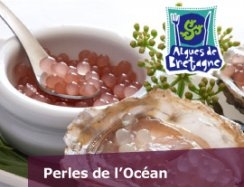
\includegraphics[scale=0.5]{Illustrations/PerlesOcean.jpg}
			\caption{Les Perles de l'Océan : un des projets réussis de Valorial\\(Source : Site de Valorial - Section "Projets Aboutis"\cite{ProjetsAboutis})}
			\label{PerlesOcean}
			\end{figure}

				D’autres projets sont plus axés sur la nutrition santé, comme Serofaim, un projet sur 2ans labellisé en 2006. Ce projet consiste en une étude sur les matières végétales pour produire un extrait ayant des propriétés satiétogène (qui provoque la sensation de satiété) afin de lutter contre la surcharge pondérale et l’obésité. Après avoir passé les tests de sécurité alimentaire, cet extrait végétal a pu être commercialisé à travers des compléments alimentaires. Ce projet a remporté un grand succès puisque le chiffre d’affaire s’élève à plus de 2 millions d’euros et qu’un dépôt a été déposé.
				
		\begin{figure}[!h]
			\centering
			
\includegraphics[scale=0.5]{Illustrations/Serofaim.jpg}
			\caption{Serofaim : un des projets réussis de Valorial\\(Source : Site de Valorial - Section "Projets Aboutis"\cite{ProjetsAboutis})}
			\label{Serofaim}
			\end{figure}		

				Bien entendu il n’est pas possible de faire la liste de tous les projets du pôle de compétitivité Valorial car ils sont très nombreux, mais également parce que les informations sont maintenues confidentielles avec beaucoup de rigueur car elles sont hautement stratégiques dans un contexte de concurrence industrielle.

				
		\subsection{Un baromètre de l'innovation}
		
		    Afin d’avoir une meilleure vision de l’innovation dans l’agro-alimentaire en Bretagne, Valorial et KPMG (société d’audits) ont réalisé le “1er baromètre de l’innovation” dans l’industrie agro-alimentaire en 2014. 

    Ce baromètre a été réalisé dans le but de mettre en avant les tendances du secteur en matière d’innovation, de comparer les objectifs et les attentes des entreprises, d’aider les entreprises à se situer par rapport aux autres acteurs, et de déterminer quels sont les problèmes et axes d’amélioration possibles via une étude basée sur les entreprises du pôle Valorial.

    L’innovation telle qu’elle est évoquée dans ce document est définie par l’apport d’une nouveauté, soit pour l’entreprise, soit pour le marché, soit pour le monde entier (première fois que l’élément de nouveauté apparaît, et ce dans tous les marchés et tous les secteurs d’activité). Le baromètre s’intéresse à quatre typologies d’innovation, les innovations de produit, de procédé, de commercialisation et d’organisation.

    On peut ainsi remarquer que dans notre contexte de crise économique, environ 18\% des ventes de 2009 sont liées à des produits innovant des industries agro-alimentaires, ce qui est supérieur à la moyenne des industries françaises. Le territoire possède un nombre très important d’établissements de recherche et compte plus de 6000 scientifiques, 820 enseignants-chercheurs de l’enseignement supérieur agricole ainsi que 1000 ingénieurs. Ces ressources sont pour l’instant peu exploitées par les entreprises qui ont encore du mal à se lancer dans des projets collaboratifs.

    Ce baromètre met également en avant une tendance à l’innovation pour les prochaines années avec seulement 2\% des entreprises qui prévoient une réduction de l’activité d’innovation. Il semble cependant qu’un certain nombre industriels fait encore une distinction entre les innovation de marché et les innovations en R \& D or c’est bien la combinaison des deux qui est nécessaire.

    Bien qu’aucune entreprise n’exclut l’innovation de stratégie, 60\% ne la considère que comme un axe d’étude parmi d’autres. Sur ce point ce sont les petites entreprises qui semblent porter plus d’intérêt à l’innovation comme vecteur de réussite.

    Il y a donc une nécessité pour les industriels de continuer à s’adapter. On constate par exemple que les effectifs des entreprises ne sont pas assez impliqués dans le processus d’innovation, qu’une entreprise sur deux ne connaît pas son propre budget dédié à l’innovation, et de manière général l’absence d’outils informatique indispensables pour les suivis de projet.

\chapter{Une innovation limitée}

	\section{Une innovation pas vraiment optimale}
	
		\subsection{Une vision trop portée sur le produit}
			Au delà des raisons historiques qui avaient pour but de relancer l’autosuffisance du pays, l’agriculture et toute l’industrie agro-alimentaire Bretonne ont subi depuis quelques décennies une modernisation massive. En effet, la région Bretonne ne disposant que de peu de terres arables, le développement de l’agriculture hors-sol a été l’un des développement phare de la région. 
			
			Dans la foulée, une majeure partie des techniques de génétique améliorée ont été développées en Bretagne. Au final, la greffe a pris puisque cette région centralise 30 \% des volailles et 50 \% des porcs consommés au sein de l’hexagone, ce qui représente une part important de l’économie de la région et est presque devenu symbolique.
			
			Mais ce développement s’est fait au mépris de l’environnement, les quotas de pêche et les considérations environnementales ont donné un sérieux coup de frein, notamment le taux de nitrates et l’arrivée des algues vertes qui ont stoppé l’extension des élevages.
			
			Ainsi, devant cette problématique d’expansion, les élevages se sont spécialisé dans le modèle dit “en batterie”, qui consiste à optimiser le nombre de bêtes élevées dans un environnement donné. Ces élevages sont vivement critiqués par les associations de défense des animaux  et ont été soumis à des législations dans certains pays comme la Suisse ou l’Allemagne. En Bretagne, seules les directives européennes font loi et les élevages n’en tiennent pas toujours compte, comme en témoigne cet article tiré de 30 millions d’amis\cite{BretagnePoussinsBroyesEtouffesDansCouvoir} : “Des poussins étouffés dans des sacs-poubelle, broyés vivants ou agonisants dans les bennes à ordures. C'est ce que révèle une vidéo publiée ce mercredi 12 novembre 2014 par l’organisme de protection animale L214.”
			
			\begin{figure}[!h]
			\centering
			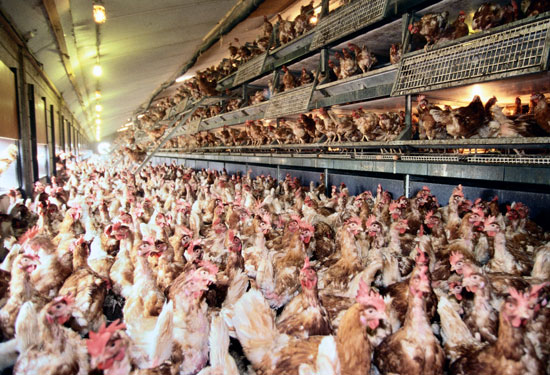
\includegraphics[scale=0.75]{Illustrations/PouleBatterie.jpg}
			\caption{L'élevage en batterie, une façon de faire de plus en plus controversée\\(Source : Wikipedia)}
			\label{PouleBatterie}
			\end{figure}
			
			Dans le cadre de notre travail avec le pôle de compétitivité Valorial, nous avons pu constater d’après leur base de données (BDD) recensant tous leurs projets traités jusqu’à maintenant, que la majeure partie de ces innovations concernaient la sécurité des consommateurs. 
			
			En effet, selon la BDD, 27\% des projets ont pour thème la santé et la nutrition. Ajoutant à ce chiffre les 32\% des projets  organisés autour de la qualité et de la sécurité des aliments, nous obtenons au total 59\% de projets qui ont pour but le bien-être du consommateur, laissant alors les autres thèmes se partager les 41\% restant. Nous devons aussi annoncer que sur les 10 projets les plus financés, 9 font partie des deux thèmes précédents, montrant ainsi l’importance accordée à la sécurité des consommateurs par les différents financeurs publics ou privés des projets de Valorial.
						
		\subsection{Un processus d'innovation parfois sans prise de recul}
			
			Nous avons expliqué précédemment la plus grande tendance de l’innovation dans l’industrie agro-alimentaire Bretonne, à savoir les innovations portées sur le produit, sa production, sa qualité, sa transparence. Peut-être que ce n’est pas ce qu’il faut à la région pour sortir de la crise.
			
			En effet, cette ligne de développement productiviste a causé des ravages au niveau environnemental. Les pesticides et les engrais chimiques utilisés massivement dans les cultures de la région déversent du nitrate dans les sols et ainsi les eaux. En trente ans, le taux de nitrates dans les rivières Bretonne a doublé, rendant parfois l’eau impropre à la consommation et participant à la prolifération d’algues vertes\cite{NitratesAlguesVertesBretagne}. Ces algues représentent un risque pour la santé humaine, leur décomposition entraine le rejet d’hydrogère sulfuré, qui est un gaz toxique. Il faut s’avoir qu’il s’en échouent entre 40 et 70 000 m3 chaque année et que le coût du ramassage s’élève à près de 500 000\euro.
			
			Les agriculteurs sont blamés car ils utilisent des engrais chimiques sur lesquels ils subissent des restrictions mais c’est le modèle économique qui veut celà. En effet, ce sont les agriculteurs qui en sont les premières victimes avec un salaire annuel moyen de 12 500\euro, l’avant denière position en terme de rémunération dans toute la France\cite{AlguesVertesNouvellePreuveRavagesProductivismeAgricole}. Malgré l’intensité de production, parfois au détriment des lois sanitaires et de protection des animaux, les agriculteurs peinent à gagner correctement leur vie.
			
			
			Le remembrement, qui est une innovation un peu plus ancienne (années 60-70) et qui consistait à rassembler et regrouper des terres cultivables pour les agriculteurs afin de les rendre plus accessibles et plus vastes, a aussi causé des ravages environnementaux. En effet, ce sont des milliers de kilomètres de haies et de talus qui ont été rasés et qui ont perturbé l’écosystème. Cette pratique a causé :
			\begin{itemize}
				\item des innondations
				\item parfois des torrents de boue
				\item l’assèchement de certains point d’eau
				\item la destruction du paysage de la région : le bocage, qui est la séparation des champs par des haies ou des talus de terre
				\item l’érosion des sols et leur appauvrissement
			\end{itemize}
			
			Autant de conséquences désastreuses sur l’environnement.	
			
			Mais au delà des innovations destructrices de l’environnement, les innovations développés dans la partie précédente, à savoir celles qui consistent à agir sur le produit en lui même, sa productivité, ses apports, la sécurité alimentaire, ne sont peut-être pas la bonne solution au problème économique du secteur.
			
			La consommation de viande de la région est plus coûteuse que celle importée, malgré les coûts de transport. Cette constatation amène une question qui peut se résumer ainsi : ne vaudrait-il pas mieux produire une viande de qualité et la vendre légèrement plus chère plutôt que de continuer à lutter contre les importation de viande de basse qualité et à faible coût alors qu’il est presque impossible de rivaliser ?
			
			La communication laisse également à désirer dans le secteur de l’agro-alimentaire de façon générale. Nous voyons très peu de publicité sur les produits de la région, quelques entreprises sont présentes comme les poulets loué qui essayent justement de répondre à la question précédente et vantent leur viande de qualité, qui se vend plus cher mais à juste prix.
			Certains produits étant délaissés, comme par exemple l’artichaut, les entreprises se lancent dans des campagnes de publicité décalés pour attirer l’oeil du consommateur, par exemple la publicité très “hot” de Prince de Bretagne.
			
		\subsection{L'agro-alimentaire, une industrie retardataire}
			Lorsque l’on pense au monde de l’agro-alimentaire, la première pensée que l’on a se rapporte majoritairement à l’agriculture. Qui dit agriculture, dit ferme, fermier, boue, charette et moissonneuse batteuse, dans l’esprit populaire.
			
			Malgré la modernisation colossale de l’agriculture au cours des 40 dernières années, ce stéréotype du monde agricole n’a pas beaucoup changé, pourtant on peut comparer certaines exploitations agricoles à de vraies usines, aux normes d’hygiène très strictes. Pourquoi cette image n’a-t-elle pas changé ?
			
			Tout d’abord, il faut resituer le contexte historique, plus particulièrement le contexte d’après guerre dans les années 50-60. La Bretagne était alors une région marginalisée et très en retard au niveau économique. L’électricité n’y est pas complètement installée et les voies de transport, particulièrement les voies ferrés, sont vétustes. L’agriculture est archaïque, ce sont de petites exploitations de subsistances très peu mécanisés.
			
			Ce n’est qu’au retour de la guerre que les paysans Bretons, enrolés dans des fermes allemandes, modernes et productivistes, vont se rendre compte du retard de leurs exploitations. Cette prise de conscience alliée au besoin de relancer l’économie et la production agricole du pays a permis de débloquer des aides considérables pour la région. Ainsi, le socialiste breton François Tanguy-Prigent, ministre de l'Agriculture dans le gouvernement d'union nationale du général de Gaulle, crée un statut pour le fermage et encourage le développement des organisations paysannes. L'Église n'est pas en reste, via la puissante Jeunesse agricole chrétienne (JAC), très implantée dans la péninsule. La JAC va entreprendre un effort sans précédent d'éducation et de formation des paysans. Elle fournit aussi des cadres qui se révéleront d'habiles négociateurs. Il faut enfin souligner le rôle du Comité d'études et de liaison des intérêts bretons (Célib) qui travaille à désenclaver la Bretagne et développer son territoire\cite{ModernisationAgricultureBretonne}. Entre 1962 et 1975, la population agricole de la région a triplé, alors qu’elle a à peine doublé en France.
			
			Cette modernisation de l’agriculture a été très bénéfique pour le secteur de l’agro-alimentaire Breton, plaçant la région en première position au niveau de la production grâce à ses infrastructures très productivistes comme l’élevage en batterie. Mais malgré tous ces efforts, les petites infrastructures peinent à se mettre à la page, surtout au niveau des innovations récentes. 
			
			En effet, bon nombre d’agriculteurs sont regroupés au sein de coopératives mais ils sont encore nombreux à ne pas utiliser l’outil informatique, devenu une des bases du système économique quel que soit le secteur d’activité\cite{FAIPeuInteresses,AdoptionTICAgricole}. Il n’y a pas que le fait d’informatiser ses revenus, sa production ou consulter les prévisions météorologiques, cet outil permet de consulter les tendances des réseaux sociaux, de créer un site web pour son entreprise voire de proposer des ventes en ligne comme le site \url{http://www.bienvenue-a-la-ferme.com/} qui permet à tous de trouver le producteur le plus proche de chez soi.
			
			C’est autour de cette problématique que se sont développés certaines entreprises comme \url{http://www.mychefcom.com/} qui sont spécialisés dans l’accompagnement des entreprises agro-alimentaire dans leur campagne de développement digital. Monsieur Le Bayon, Community Manager dans l’entreprise Mychefcom citée précédemment, nous a par exemple raconté que certaines grandes entreprises avec qui ils travaillent lui ont bien précisé de contacter le producteur par téléphone ou par courrier car il ne disposait pas d’un ordinateur personnel ou professionnel. raconté que certaines grandes entreprises avec qui ils travaillent lui ont bien précisé de contacter le producteur par téléphone ou par courrier car il ne disposait pas d’un ordinateur personnel ou professionnel. Ces entreprises proposent donc des services comme le consulting en stratégie digitale, qui est l’accompagnement de l’entreprise dans la mise en place de sa stratégie commerciale sur le web ,la création d’un site web, une liste de contacts mail ou bien d’implanter l’entreprise sur les réseaux sociaux.
			
			Nous pouvons donc constater que le domaine de l’agro-alimentaire est, malgré certaines structures innovantes comme le pôle de compétitivité Valorial, un secteur en retard au niveau de l’innovation. Pour autant, cette tendance commence à s’inverser et de plus en plus d’entreprises et de producteurs se lancent dans l’exportation à l’étranger, la modernisation de leur communication et s’ouvrent petit à petit au monde de l’industrie moderne.
			
	\section{L'innovation, inaccessible pour certains}
		L’innovation est indissociable de la recherche. Or la recherche a un certain coût. Et ce fameux coût, toutes les entreprises ne sont pas capables de l’assumer. Car ce coût peut être financier, humain ou technologique. Et souvent pour palier à un des manques, les entreprises ont recours à des laboratoires pour les aider dans leurs projets.
		
		\subsection{Les contreparties à l'innovation}
		
		Toutes les entreprises cherchant à innover, elles visent un certain retour sur investissement. Ce gain n’est malheureusement pas certain car il y a un risque d'échec. Par exemple, le consommateur peut ne pas être attiré par le nouveau produit, le nouveau traitement des aliments revient plus cher et compliqué à l’utilisation que prévu, ... Mais ce risque est très souvent minimisé via “recherche d’applications et test de marché, sourcing technologique et expérimentation, recherche d’antériorités, contexte réglementaire et  normatif…”\cite{GlobalVision}. Ces techniques peuvent être mises en place via des simulations ou des expériences qui ne génèrent pas un trop gros coût.
		Mais ces différentes prises d’informations peuvent conduire à une fuite des informations. Ces fuites sont un gros problème car souvent l’idée même peut être à la base d’un très gros revenu.
		
		Enfin, innovation nécessitant une recherche spécifique, elle a un coût. 
		
			
		\subsection{Le coût élevé}
		Il existe de nombreuses aides pour toutes les entreprises souhaitant “innover”. Toutes ces aides passent par la constitution d’un dossier qui sera étudié et validé lors de l’étude de faisabilité. Si il est validé, les entreprises prenant part au projet se verront dans l’obligation de soutenir le projet lors des différentes phases de sont développement : recherche et développement, lancement du nouveau produit/service, commercialisation et exportation. Pour toutes ces étapes, il y un certain nombre d’organismes qui s’en occupent, comme par exemple France Active, Ubifrance ou Valorial\cite{AidesInnovation}. 
		
		A terme, l’objectif idéal serait d’avoir un coût pour toutes les étapes annexes au vrai projet serait dans l’ordre de 1 à 6\% du coût total du projet. Mais en réalité, toutes ces choses additionnelles mais non pas superflues, comme part exemple l’étude de marché, représentent entre 10\% et 15\% du montant du projet. Il arrive que dans certains cas, comme dans l’insdustrie des cosmétiques, que ce budget atteigne 55\% du projet ! Pour pouvoir mener à bien son projet innovant, il faut d’abord savoir comment répartir son budget sans négliger toutes ces étapes annexes. Le plus souvent, une PME n’a pas forcément les compétences pour analyser et budgétiser ces sur-coûts, donc ils font appel à des sociétés externes qui aident à la création du projet mais aussi qui alourdissent le coût total.
				
		\subsection{Une vision de spécialisation pour les petites structures}
		
		Les petites entreprises ont un budget limité, donc afin de mener une recherche il faut qu’elle aie un coût raisonnable. De plus, avoir un coût limité veut dire aussi qu’il y a un champs de recherche limité. Les PME gagnent souvent plus à se spécialiser dans un domaine plutôt que de se développer sur plusieurs marchés à la fois. Aussi les PME n’ont pas forcément des contacts pour faire de la recherche dans un domaine ou un autre. Ils leur faut donc du temps afin de pouvoir mettre en place tous les acteurs afin de faire aboutir leur projet de recherche. Il existe des solutions qui permettent de mettre en contact toutes les parties pouvant être intéressées comme Valorial. Ces solutions sont de grandes aides au développement d’un projet. De plus, au travers de ces grands groupes, les projets peuvent être mis en avant et valorisés. Ainsi ils auraient une meilleure visibilité sur le marché. 
	
	\section{Les solutions actuelles}
		Aujourd’hui, plusieurs solutions existent pour améliorer la pratique de l’innovation dans les entreprises. Afin de mieux cibler ce qui peut être fait, nous commencerons par étudier l’avantage qu’apporte les pôles de compétitivité et ce qu’il peuvent amener à l’avenir. Ensuite, nous verrons les nouveaux processus d’innovations adaptés à l’agro-alimentaire. Pour terminer, nous nous pencherons sur les avancées effectuées en matière de recherche scientifique.
		
		\subsection{Les pôles de compétitivité}
		Tout d’abord, les pôles de compétitivité constituent un facteur important en ce qui concerne l’innovation.
		
		Pour commencer, il est important de rappeler la spécificité des pôles de compétitivité, organisations créées il y a dix ans suite au Rapport Blanc donnant en 2004 la priorité à la croissance et à la compétitivité dans l’économie nationale\cite{RapportBlanc}. Il existe quatre types de systèmes collaboratifs, se différenciant selon qui souhaite la collaboration et qui collabore, comme illustré à la Figure  \ref{ComparaisonSystemesCollaboratifs} ci-dessous.
	
		\begin{figure}[!h]		
		
		\vspace{11pt}
		\begin{center}
		\begin{tabular}{|M{110pt}|M{100pt}|M{100pt}|}
			\hline
			& \textbf{Collaboration voulue par les acteurs eux-mêmes} & \textbf{Collaboration reconnue et renforcée par les pouvoirs publics}\\
			\hline
			\textbf{Tous les partenaires sont des entreprises} & Districts industriels & Systèmes Productifs Locaux (SPL)\\
			\hline
			\textbf{Partenaires d'organisations variées (entreprises, universités, ...)} & Cluster & Pôles de compétitivité\\
			\hline
		\end{tabular}
		
		\caption{Les pôles de compétitivité, une forme de collaboration inter-organisationnelle \\(Source : Pôles de compétitivité, Propos d'étape. Revue Française de Gestion\cite{PoleCompetitivite})}
		
		\label{ComparaisonSystemesCollaboratifs}
		\end{center}
		\end{figure}
		
		Ainsi, les pôles de compétitivités diffèrent de leurs semblables par le large éventail d’organisations concernées, mais aussi par son origine gouvernementale.
		Ensuite, il est intéressante de savoir comment fonctionne un pôle de compétitivité. Suite à une étude menée par Thomas Froehlicher et Franck Barès sur plusieurs agglomérations et régions, dont la Bretagne, a permis de dessiner un fonctionnement\cite{PolesCompetitiviteClusters}. Dans un premier temps, les pôles de compétitivité se renseignent au travers de veilles. Grâce à cela, ils deviennent capables d’anticiper les futures tendances. Ils peuvent donc projeter leur activité dans ce futur et se restructurer en fonction de cela. Le pôle de compétitivité qui a suivi ces étapes devient alors capable d’inventer les produits de demain. Ces produits sont ensuite fabriqués par les entreprises à l’origine de projets.
		Ces pôles sont d’ailleurs, pour la plupart, relativement efficaces. Sur les 71 pôles de compétitivité français, 39 ont réussi à respecter leurs objectifs, tandis que seulement 13 devaient être restructurés en 2008\cite{PolesCompetitiviteClusters}. Pour le pôle de compétitivité breton Valorial, ce sont pas moins de 250 projets qui ont été labellisés en moins de dix ans\cite{ProjetsValorial}. Parmi eux, on trouve le projet SpectraG qui a permis à l’entreprise Valorex de mettre en place une méthode pour prédire les acides gras provenant des tissus adipeux dans les élevages, et donc d’améliorer la qualité des produits en termes de nutrition\cite{ProjetsAboutis}. Un nombre conséquent d’autres projets ont pu être menés à rien en partie par l’action de pôles de compétitivité sur toute la France.
		Pour autant, ce ne sont pas les pôles de compétitivité qui ont permis aux entreprises d’entrer en contact les unes avec les autres. En effet, un tissu industriel était déjà présent avant 2004. Malgré tout, la création de ces pôles aura permis le renforcement de ce phénomène. On voit par ailleurs que, depuis leur création, les pôles de compétitivité sont passés d’une optique plutôt gouvernementale à une place de catalyseur dans l’économie locale.
		D’autant plus, les actions de ces pôles sont parfois limitées, et le manque d’influence sur la distribution des ressources se fait sentir. On constate par exemple que certaines grosses entreprises sont capables de se passer de l’aide des pôles sans avoir pour autant une réelle organisation dans l’innovation, tandis que des petites structures innovantes peuvent se retrouver bloquées à cause du manque de ressources qui leurs sont allouées par les partenaires.
		C’est pour cela que les pôles de compétitivité tendent à se rapprocher d’un écosystème de croissance, qui permettrait d’avoir une plus grande emprise sur les ressources qui passent par l’organisation, et de renforcer encore plus efficacement l’innovation.
		
		En conclusion, les pôles de compétitivité revêtent une importance toute particulière au sein de l’économie, en permettant aux entreprises d’innover plus et mieux.
				
		\subsection{Les nouveaux modèles d’innovation}
			Suite aux problèmes qu’à l’industrie agro-alimentaire à se renouveler, plusieurs modèles ont été mis aux points dans le but de faciliter l’innovation dans un secteur considéré comme mature et à faible taux d’innovation.
			
			En premier lieu, il convient d’expliquer d’où provient le besoin en termes de nouveaux modèles d’innovation. Dans l’économie actuelle, l’industrie agro-alimentaire est considérée comme une industrie mature, puisqu’elle n’offre plus beaucoup de perspectives d’évolution. En réalité, la plupart des innovations qui peuvent servir cette industrie ont déjà été produites. C’est pour cela que l’innovation paraît depuis quelques années être peu avantageuse pour les entreprises du secteur. Cela a produit un désintéressement de la part de beaucoup d’acteurs, faisant ainsi de cette industrie une industrie à faible taux d’innovation. Or, il est aujourd’hui possible d’apporter des innovations importantes et rentables, comme l’ont montrés de nombreuses entreprises.
			Dans l’optique de relancer l’innovation dans l’industrie agro-alimentaire, trois principaux modèles ont été proposés, tous dans une vision d’Open Innovation (innovation plus ouverte et collaborative)\cite{OpenInnovation}. Le premier d’entre eux est Sharing is Winning (littéralement, “Partager c’est Gagner”)\cite{SiW}. Ce modèle se base sur la coopération entre partenaires de natures diverses pour réussir. Même s’il est utilisé depuis quelques années, ce modèle est défini par Traitler et Saguy en 2009. Il a pour but de partir d’innovations proposées par les consommateurs, puis de les dispatcher sur toute la filière de production (fournisseurs et acheteurs compris)\cite{OIFr}. Un exemple d’entreprise ayant adopté ce modèle est le groupe Nestlé\cite{NestleOI}, qui depuis 2007 met en place ce mode de fonctionnement en partenariat avec Cargill, BASF et l'Université Polytechnique de Lausanne. Le processus d’innovation s’en est trouvé accéléré de manière sensible.	
			
			\begin{figure}[!h]
			\centering
			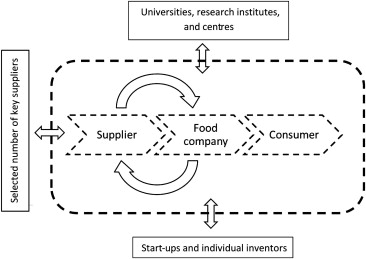
\includegraphics[width=10cm]{Illustrations/Schema_SIW.jpg}
			\caption{Le modèle Sharing is Winning \\(Source : Models of adoption of open innovation within the food industry\cite{OpenInnovation})}
			\label{ImageSiW}
			\end{figure}
			
			Un autre modèle proposé est le food-machinery framework (littéralement, “Structure du mécanisme alimentaire”). Une illustration est donnée plus bas (Figure \ref{ImageFMF}) Institué par Bigliardi, Bottani et Galati, il s’intéresse à la chaîne de production et aux acteurs qui l’entourent\cite{FMF}. Il est assez facile à mettre en œuvre pour de grosses structures, puisqu’elles ont par avance un réseau leur permettant de collaborer plus simplement et plus souvent.
			
			\begin{figure}[!h]
			\centering
			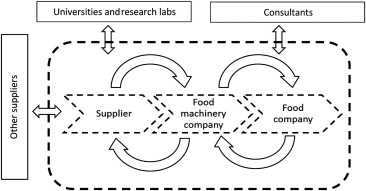
\includegraphics[width=10cm]{Illustrations/Schema_FMF.jpg}
			\caption{Le modèle "Food-machinery Framework" \\(Source : Models of adoption of open innovation within the food industry\cite{OpenInnovation})}
			\label{ImageFMF}
			\end{figure}
			
			Enfin, le modèle Want, Find, Get, Manage (“Vouloir, Chercher, Obtenir, Gérer”), voir Figure \ref{ImageWFGM}, se veut très ouvert sur le fonctionnement existant. Ce modèle, initialement proposé par Slowinski\cite{WFGM}, propose de s’intéresser, quel que soit le problème, à ce que d’autres acteurs ont déjà mis en place. Contrairement au précédent, ce modèle est plus accessible pour les petites structures, puisqu’il suffit de se renseigner sur ce qui existe plutôt que de butter sur un problème. Il est même préférable de ne pas avoir trop de relations à gérer dans ce modèle.

			\begin{figure}[!h]
			\centering
			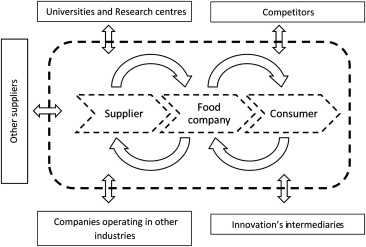
\includegraphics[width=10cm]{Illustrations/Schema_WFGM.jpg}
			\caption{Le modèle Want,Find, Get, Manage \\(Source : Models of adoption of open innovation within the food industry\cite{OpenInnovation})}
			\label{ImageWFGM}
			\end{figure}
			
			Ainsi, même si l’industrie agro-alimentaire peine à se renouveler, il existe aujourd’hui des solutions, gravitant autour de l’Open Innovation. Il apparaît donc que l’industrie agro-alimentaire nécessite avant tout la mise en place d’un collaboration.
			
		\subsection{Les avancées en matière de recherche}
			Les solutions précitées ne sont bien évidemment pas les seules à pouvoir redresser la barre de l’innovation dans l’industrie agro-alimentaire. En parallèle avec celles-ci, plusieurs autres pistes existent. Nous commencerons par voir ce qui est apporté par les autorités publiques. Nous parlerons ensuite des nouvelles avancées dans la recherche.
			
			Pour commencer, plusieurs solutions pour améliorer l’innovation dans le secteur ont été proposées par les pouvoirs publiques. L’OCDE a présenté, en 2009, un rapport \cite{OECD} faisant suite à des observations faites sur la période 2007-2008. Même si certaines de ces ouvertures ont déjà été exploitées (les bioproduits, par exemple, représentent aujourd’hui un marché en vogue). Pour autant, des domaines comme celui des aliments fonctionnels (aussi appelés alicaments) restent encore trop peu utilisés. Ainsi, même si quelques entreprises portent des projets de cet intérêt, elles sont une exception. Cela s’explique par le fait qu’il est difficile de créer des aliments avec un effet bénéfique sur la santé, et que le coût de ces aliments est élevé. Pourtant, la filière des aliments fonctionnels représente à la fois un bénéfice pour la santé publique, elle est également très fructueuse pour les entreprises (75,5 milliards de dollars de la création à la fin du siècle dernier jusqu’à 2009). Cette filière, lancée en France par Unilever et sa margarine réduisant le taux de cholestérol (encore vendue sous le nom de Fruit d’Or ProActiv)\cite{FruitDOr}, est donc l’une des priorités publiques depuis quelques années en matière d’innovation agro-alimentaire. Le gouvernement français se penche également de manière significative sur le problème de la communication dans l’industrie agro-alimentaire. Ainsi, il propose de valoriser les produits français avec les logos Viande de France cités plus tôt, mais cherche aussi à instituer une simplification à l’égard des consommateurs avec la notation par étoiles sur les pièces bouchères\cite{EtoilesViande}. 

			\begin{figure}[!h]
\centering
			
\includegraphics[width=5cm]{Illustrations/Alicament.png}
			\caption{L'alicament, ou la médication par l'alimentation}
			\label{alicament}
			\end{figure}
			
			

			Ensuite, puisque l’innovation est un problème majeur dans l’actualité, une importance toute particulière lui est donnée par l’État, ce qui a mené entre autres à la création de pôles de compétitivité axés sur l’agro-alimentaire, au nombre de 10 sur les 71 pôles labellisés dans le pays\cite{CompetitiviteGouv}. Cet appui donné aux pôles de compétitivité agro-alimentaires crée donc une synergie, comme expliqué plus tôt. Mais cette synergie s’ajoute aujourd’hui à la prise de conscience de nombreux acteurs, ce qui améliore de manière considérable l’innovation. Il reste néanmoins à sensibiliser tous les acteurs de manière efficace et définitive, dans l’optique d’obtenir un fonctionnement réellement adapté pour la mise en place d’une stratégie d’innovation au niveau national.

			Enfin, la recherche propose elle aussi des solutions d’avenir. En se tournant vers de nouveaux domaines, plus porteurs, tels que la qualité des aliments, la santé et la nutrition. Ainsi, le pôle agronomique cherche à trouver des méthodes plus respectueuses de l’environnement, et permettant la production la plus écologique possible\cite{PoleAgroOuest}. Tout cela a pour intérêt de renforcer à la fois la qualité du produit (en terme de risques sanitaires et de nutrition). Les centres de recherche comme le pôle agronomique et l’INRA (Institut National de la Recherche Agronomique) se mettent également à développer des réseaux dans le but d’accompagner les entreprises et l’industrie qu’elles portent de façon plus efficace. À cette fin, le pôle agronomique de l’Ouest est en relation avec les pôles de compétitivité Valorial en Bretagne et Végépolys en Pays de Loire, tout en participant activement à la mise du pôle Mer\cite{PoleAgroOuest}. 

  			 Pour conclure, on remarque que tous les acteurs ont un rôle à jouer dans la mise en place d’une réelle innovation au sein de l’industrie agro-alimentaire.

\chapter*{Conclusion}
\addcontentsline{toc}{chapter}{Conclusion}
	Pour conclure, nous pouvons affirmer, d’après ce que nous avons dit, que l’agro-alimentaire français présente des particularités intéressantes. En effet, même si sa compétitivité est dans une tendance plutôt à la baisse, ainsi que l’emploi, au profit d’une mise en valeur de la compétitivité via l’export et la technologie, qui restent des activités porteuses. La Bretagne présente une différence importante dans cet agro-alimentaire français. En effet, grâce à sa place privilégiée pour ce qui est de la géographie et de l’économie, et à la présence de multiples secteurs d’activités, elle représente un poids très important au cœur de l’industrie agro-alimentaire mondiale. Depuis quelques années, pourtant, la crise frappe de plein fouet ce secteur. Même si, grâce à situation, ma Bretagne se porte mieux, les différentes actions menées ne suffisent pas à elles seules, et il est nécessaire de prévoir des solutions d’avenir pour redresser ce bilan mitigé.
  
    Afin de remédier à cette crise, l’innovation semble aujourd’hui être un remède miracle.  Celle-ci se décline sous diverses formes, selon les différents échelons auxquels elle peut exister, à savoir la production, la communication et les ressources. Pour bien innover, les entreprises doivent donc faire de la recherche, mais aussi tenir compte de leur environnement, afin de mettre en place les produits de demain. C'est un des objectifs du pôle Valorial, qui apporte un nouveau souffle à l'innovation dans l'industrie agro-alimentaire bretonne.

    Malheureusement, cette innovation ne donne pas toujours les résultats escomptés. Il arrive régulièrement qu’elle ne soit pas faite de façon optimale, ou qu’elle n’apporte pas de réponses aux vrais besoins du marché. Cela arrive lorsqu’une entreprise s’intéresse trop spécifiquement au produit. Le temps compte aussi, puisque nombre de produits innovants arrivent trop vite, sans recul, sur le marché, tandis que d’autres arrivent à la traîne. Un autre problème majeur sur l’innovation est l’avantage procuré aux grandes entreprises, car elle implique de nombreuses contreparties à l’image du coût élevé nécessaire à la mise en œuvre d’un processus d’innovation.
    
    Pour compenser les problèmes que cela pose, des solutions existent. À l’heure actuelle, les acteurs de l’industrie agro-alimentaire se tournent vers les pôles de compétitivité, les nouveaux modèles d’innovation, ainsi que vers les avancées de la recherche.
    
    En raison de tout cela, nous pouvons dire que le monde de l'agro-alimentaire se trouve aujourd'hui dans une posture plutôt mauvaise, avec néanmoins quelques exceptions. L'innovation semble d'ailleurs être l'une des principales raisons pour expliquer la présence de ces exceptions, mais elle reste un outil souvent mal utilisé, car mal maîtrisé. Depuis plusieurs années, pourtant, de nouveaux acteurs émergent, et avec eux de nouveaux modèles économiques, plus portés sur l'innovation, apparaissent. Ceux-ci laissent entrevoir de futures innovations apportées de manière plus réfléchie.
    
    Une question demeure cependant en suspens. Il reste à savoir si les grands acteurs de l'industrie agro-alimentaire, à savoir les entreprises, seront capables de réagir rapidement et de façon adéquate pour redresser la barre de l'économie à laquelle ils appartiennent.

\appendix
\chapter{Interview de Christophe JAN, chargé de communication chez Valorial, et de Régis DEL FRATE, ingénieur projet chez Valorial}
\label{Interview}

	Interview réalisée le 16 Janvier 2015

	\textbf{\\Comment se déroule un projet et autour de qui cela gravite-t-il ?}

	\emph{Christophe JAN}

	C’est très variable, certains des projets qui arrivent sont déjà entièrement finis, parce qu’ils sont proposés par des partenaires de projets ayant déjà été en relation avec nous, et d’autres non. En ce moment, nous réfléchissons sur le moyen d’intéresser les industriels.
Pour résumer, on peut partir soit d’idées soumises par des industriels sans aucun partenaire ni thématique précise, soit d’idées que nous soumettons aux industriels pour voir comment ils vont s’associer à d’autres industriels, des laboratoires de recherche.

	Chaque projet contiendra à minima deux partenaires économiques dans l'agro-alimentaire, au sens large. C’est-à-dire qu’ils peuvent être de grands groupes adhérents chez Valorial, des transformateurs, des équipementiers, des apporteurs de solutions technologiques. À partir du moment où chaque partenaire apporte ses compétences pour la R \& D, ils peuvent en faire partie.


	À ces porteurs de projet, on associe des structures académiques ou techniques, qui vont représenter la partie recherche du projet.

	La typologie du projet, elle, varie en fonction des partenaires, de la nature des travaux à évaluer. Il y a plusieurs types de budgets possibles selon les projets. L’année dernière, le plus petit budget était de 200 000 €, et le plus conséquent représentait 10 000 000 €. On a donc des typologies très différentes, des natures de projet différentes, tous très variés.

	Il y a quand même une majorité (environ la moitié) d’industriel compétitifs, qui cherchent à développer un service ou process pour le mettre sur le marché à court ou moyen terme, sachant que la durée moyenne d’un projet tourne autour de deux ans et demi, avec en moyenne cinq partenaires environ.

	Le processus déroulé d’un projet, aujourd’hui, consiste d’abord à accompagner le montage d’un projet, à partir de l’idée soumise, avec la réflexion avec les partenaires, aux questions sur le but du projet, à ce qu’il peut apporter à l’industrie agro-alimentaire. Puis on s’intéresse à la direction qu’il faut prendre, aux bon partenaires à choisir; mais il peut aussi y avoir un partenaire qui arrive en sachant avec qui il veut travailler, ce qui permet de ne pas avoir à rechercher les partenaires.

	Le coeur de métier de Valorial est donc d’accompagner les projets, mais aussi d’apporter une ingénierie financière et une vision aguerrie sur le projet. L’idée reste quand même d’aider les porteurs de projets à obtenir des soutiens financiers.

	\textbf{\\Les idées de projet peuvent-elles venir de l’extérieur ?}
    
	\emph{Christophe JAN}

	Oui, ça peut être des industriels qui émettent une idée, un besoin auquel ils ne peuvent pas subvenir eux-mêmes. Ça peut aussi être des structures académiques, qui cherchent à accompagner un travail de recherche pour transformer une recherche fondamentale, théorique en une recherche plus concrète, plus compétitive, sur une expérience grandeur nature.

	\textbf{\\Comment faites-vous pour mettre les acteurs en correspondance ?}

	\emph{Christophe JAN}
    
    On a différentes “animations” au niveau du pôle, appelées commission thématiques, dans lesquelles peuvent intervenir des chercheurs, qui vont présenter leurs recherches et tenter de savoir si des industriels dans l’agro-alimentaire sont interessés par ces recherches.

	\textbf{\\Et vous intervenez sur un type de projet précis ?}

	\emph{Christophe JAN }
  
    Oui. L’idée porte sur des projets d’innovation et de R \& D. Le but est d’accompagner des projets innovants. Dans le cas où un industriel cherche à se moderniser à partir de ce qui a pu être fait par d’autres, cela ne concerne pas le pôle. Le but de Valorial est vraiment d’apporter une recherche et de nouvelles compétence au monde de l’agro-alimentaire en lui-même. En général, toute cette activité est encadrée avec des consortiums, des accords de confidentialité, des accords de PI (Propriété Intellectuelle), etc. 

	\emph{Régis DEL FRATE}
 
    Il faut juste rappeler que contrairement à l’innovation classique, Valorial favorise l’innovation plus collaborative. Cela implique évidemment un “mix” entre chercheurs et industriels. 

	\textbf{\\Comment faites-vous pour avoir autant de projets ?}

	\emph{Régis DEL FRATE}
	
    Après, il y a tout un tas de dispositifs pour arriver à cette émergence de projets : des réunions de travail, des groupes thématiques par filières ou sous-filières.

	\emph{Christophe JAN}

    Il y a aussi des appels à projets.

	\emph{Régis DEL FRATE}

    À partir de ça, on a des réseaux, des “pipes” qui font remonter les projets jusqu’à Valorial. Une fois qu’ils y sont arrivés, on vérifie, dans un comité de labellisation, qui est indépendant, le bien-fondé du projet, on vérifie qu’ils sont des projets collaboratifs, pour pouvoir le labelliser. Il peut aussi être colabellisé entre plusieurs pôles, s’il y a lieu.

	\textbf{\\Par “comité de labelisation indépendant”, vous entendez que cela est géré par des structures extérieures ?}

	\emph{Christophe JAN}

    En fait, c’est un consortium de 12-13 personnes qui viennent à titre personnel, et représentant différentes structures : l’INRA, l’École d’ingénieurs de Caen, la Chambre de Commerce, la Chambre d’Agriculture, la technopole Rennes Atalante. Il y a aussi le président des centres techniques bretons, … Ce sont tous des gens qui n’ont pas d’intérêts personnels dans le projet. Dans le cas où un conflit d’intérêt serait observé, la personne concernée ne serait pas autorisée à labeliser le projet. On connaît au préalable les attentes des labelisateurs, donc on essaie de leur apporter des projets qui les intéressent. En fait, vu que la plupart du temps, ce sont des idées qui arrivent jusqu’à nous, on tente de transformer ces idées en projets qui conviennent à ces attentes (bonnes thématiques, collaboration, …). Une fois que le projet est accepté, Valorial peut présenter le projet au nom de tout le consortium devant les financeurs potentiels. Ces financeurs potentiels sont les collectivités territoriales (Bretagne, Pays de Loire, Basse-Normandie) au travers des conseils régionaux; l’État au niveau national, et quelques autres collectivités. Si ces collectivités peuvent être interessées de par la typologie du projet, le projet leur est présenté, sinon il existe d’autres possibilités : l’État met à disposition le FUI (Fond Unique Interministériel) pour financer les projets de plus grande envergure, notamment lorsque certains des partenaires sont hors du territoire national, puisque les collectivités territoriales ne veulent alors pas (et ne peuvent pas) les suivre ni les aider.

	\emph{Régis DEL FRATE}

    Pour faire simple, on labellise les projets pour leur permettre d’accéder à des sources de cofinancement public. On est une sorte de guichet qui oriente les projets vers les partenaires qu’il faut, et aucun financement n’est proposé directement par Valorial.

	\emph{Christophe JAN}

    On organise les projets et on les facilite.

	\textbf{\\D’où proviennent, plus précisément, les financeurs ?}

	\emph{Christophe JAN }

    Comme je le disais, les financeurs sont les régions, qui ont des fonds spécifiques pour les projets collaboratifs. Ici, il y a Rennes Métropole, la technopole de Brest, les conseils généraux, la région elle-même. Parfois, le comité européen s’intéresse aussi aux projets. Et l’État propose un budget dédié, le FUI, comme on en parlait plus tôt. C’est un fond commun qui permet à chacun des ministères dont dépendent les pôles de compétitivité d’apporter un financement supplémentaire aux projets d’innovation collaborative.

	\textbf{\\Toutes les régions fonctionnent de cette façon  ?}

	\emph{Christophe JAN }

    Il ne faut pas faire de généralité. Nous parlons de Valorial, et je pense qu’il n’existe pas deux pôles de compétitivité ayant deux systèmes identiques. À part sur les projets nationaux, les fonctionnements de chacun sont très différents. Pour un projet qui serait labelisé par Valorial et qui répondrait à une certaine typologie, il ne serait pas forcément financé de la même façon par un autre pôle. Et cela dépend aussi des politiques d’innovation régionales, des schémas d’innovation, … . J’oubliais qu’il y a un autre financeur potentiel, qui est le ministère de la recherche. Sur les projets fondamentaux, pour récupérer des,connaissances exploitables dans des projets moins fondamentaux, Valorial labellise aussi des projets ANR, qui sont financés par l’Agence Nationale de la Recherche. Ce sont des projets plus fondamentaux, liés à de la recherche, de façon à ce que l’industrie agro-alimentaire s’y intéresse.

	\textbf{\\Quel est votre rôle une fois que le projet est labellisé ?}

	\emph{Christophe JAN}
	
	Après, on prend du recul, une fois que le projet est financé, à l’heure actuelle, on n’accompagne pas les projets.

	Pour l’estimation, il doit y avoir environ 100 projets en cours labellisés par Valorial. On n’a pas la ressource pour suivre ces projets. On est en réflexion pour vendre du temps d’ingénieur pour suivre ces projets, mais ce n’est pas actuellement une vocation forte au niveau du pôle. C’est une possibilité pour le développement du pôle, car aujourd’hui les pôles doivent aller de plus en plus vers du financement privé, s’autofinancer de plus en plus. Juste pour les chiffres, Valorial est actuellement financé à hauteur de plus de 60\% par des fonds publics et le reste est de la ressource privée. Et l’État demande à ce que ce rapport s’inverse.

	\emph{Régis DEL FRATE}

    Ces fonds privés proviennent des cotisations des adhérents. Chaque adhérent paye une cotisation annuelle en fonction de la taille de la structure pour avoir accès à différents services dont la labellisation des projets, de la veille, des invitations à des salons. On accompagne aussi les projets quand les produits ou les process sont terminés. On peut contribuer à la promotion de ces projets via les relations de presse, les salons, … C’est toute la partie communication.

	\emph{Christophe JAN}
	
    Et cette communication est faite au nom du projet. L’objectif est de ne pas mettre en avant un partenaire plus que les autres. Par exemple, pour le saucisson Hénaff, on ne va pas dire que c’est grâce à Hénaff mais qu’il y a tout un travail derrière. On va mettre en avant tous les partenaires qui ont permis au produit de se développer.

	\emph{Régis DEL FRATE}

    On est une espèce d’usine à projet et, en quelque sorte le “meetic” de l’agro-alimentaire.On va chercher les compétences que les entreprises n’ont pas en interne et on met en relations les partenaires.

	\textbf{\\Et vous n’apportez aucune expertise technique ?}

	\emph{Christophe JAN}
	
    Au sein de Valorial, on ne sait pas faire. On reste des généralistes, qui s’appuient sur des compétences techniques. On s’intéresse à toutes les filière agro-alimentaire, avec des thématiques nutrition, santé animale, ingrédients, emballages, marketting alimentaire, qualité, … Pour ce qui est microbiologie, chimie,... on n’a pas les compétences mais on sait qui pourrait faire pour les acteurs qui le sollicitent.

	\textbf{\\Est-ce que vous auriez des exemples de projets par rapport à cela ?}

	\emph{Christophe JAN}

    C’est assez difficile, puisqu’il y a beaucoup de typologies de projets différentes.

	\emph{Régis DEL FRATE}
	
    Il y en a énormément. Sur Rennes, je peux citer deux exemples.
    
    Le premier exemple, c’est un produit qui est sorti il y a pas de temps déjà, qui s’appelle “Les perles de l’océan”. Ce sont des billes d’algues fourrées avec des saveurs sucrées/salées. C’est un projet que l’on a accompagné, et c’est aussi notre tête de gondole. C’est un des tous premiers projets du pôle, c’est un vrai projet collaboratif, avec l’association de plusieurs compétences. Il a été primé, au SIAL, sur des salons de référence dans l’agro-alimentaire.

	\emph{Christophe JAN}
	
    Et le livrable du projet a tellement bien marché qu’il a été copié. L’idée est de pouvoir enfermer, à l’intérieur de petites billes, soit des compotes soit des purées; et il s’avère que dans les algues on trouve plusieurs composés intéressants. Le porteur de projet est venu nous voir, on l’a mis en contact avec le CEVA (Centre d’Étude et de Valorisation des Algues) et une structure d’étude plus technique. Il y avait aussi d’autres partenaires. On est dans un cas où l’association est venue naturellement. 

	On a eu un autre cas où chercheur est venu avec une technologie qui pouvait être utile pour améliorer la congélation des fruits et légumes et qui voulait voir sa technologie mise en oeuvre. On l’a mis en relation avec des personnes qui sont dans le domaine des fruits et légumes surgelés et on fait en sorte de déployer ce projet.

	Après tout ça se déroule en beaucoup plus d’étapes et dure plus d’un an et demi en l’occurrence. Il y a aussi des projets qui vont plus vite, comme des projets de valorisation de nouveaux ingrédients. On parle beaucoup de microalgues qui ont des vertus intéressantes en protéines, et donc on recherche comment valoriser ces microalgues dans des boissons pour les sportifs par exemple. On va avoir un chercheur qui vient nous voir pour valoriser sa découverte et on le met en relation avec une entreprise dans les compléments alimentaires, et un laboratoire qui a des compétences dans tout ce qui est étude de l’exercice physique en lien avec l’alimentation.
	
	Ça peut être un grand fabriquant de produits laitiers, qui fabrique des produits à l’échelle mondiale, et qui cherche comment produire des yaourts allégés, par rapport à des technologies qui existent. Donc par exemple là, on a labellisé un projet qui tourne autour de 3 000 000 € pour sortir des nouveaux yaourts allégés.
	
	C’est très vaste. Cela peut aussi être des projets qui permettent de créer des plates-formes qui vont permettre d’aider à la R \& D derrière, comme le Centre Culinaire Contemporain. C’est une structure située à Rennes qui a une partie pour le public et une partie dédiée aux entreprises, avec de la R \& D. C’est un projet que Valorial a accompagné de A à Z. C’est ce qu’on appelle des projets de plates-formes d’innovation.

	\emph{Christophe JAN}
	
    Il peut y avoir des projets plus en amont, avec des projets sur la génétique animale, sur de la sélection variétale, … Un fabriquant de chips n’a pas forcément les mêmes besoins en qualité de pomme de terre que les fabriquants de choucroute en plats préparés. Avec la sélection variétale, on sera plus à même de dire qu’une variété est plus apte pour faire des chips ou pour faire des préparations pour choucroute. Les projets peuvent aussi tourner autour des compléments alimentaires.

	\textbf{\\Chaque partenaire à l’air d’avoir son importance propre en terme de financements...}

	\emph{Christophe JAN}
	
    Dans un projet, chaque financeur est vu de façon individuelle. Chaque partenaire va avoir un financement qui provient d’un ou plusieurs financeurs, et tous les partenaires ne sont pas financés par les mêmes financeurs. 

	Si on prend deux industriels et un laboratoire, un laboratoire en Basse-Normandie, un industriel en Pays de Loire et un autre en Bretagne, on peut imaginer que le laboratoire est financé par la région Basse-Normandie, et que les industriels le sont par leurs conseils régionaux respectifs. Et on peut imaginer que le conseil régional breton finance, mais s’appuie en sur les conseils généraux du 56 (Morbihan) et du 29 (Finistère).
	
	Et, en temps normal, on retombe toujours sur les mêmes taux de financement par partenaire. Par exemple, un PME bretonne aura toujours 45 \% de financement.

	Tout partenaire de projet est financé partiellement. Un laboratoire académique est financé à hauteur des coûts additionnels, c’est à dire que l’investissement est pour le projet. Pour les industriels, on va de 25 \% d’aide à 50 \% selon la typologie du projet. Tout en sachant que l’aide est généralement plus élevée pour les petites structures. Il y a les subventions, mais il y a aussi l’avance remboursable, qui est différente. Et il y a évidemment de l’auto-financement.
  
    Pour les financeurs publics, il y a différentes façons de présenter les projets. Soit il y a un remboursement de 100 \% des coûts additionnels, c’est-à-dire des coûts supplémentaires générés par le projet, soit 40 \% des coûts totaux.

	\textbf{\\Serait-il possible d’obtenir plus de renseignements sur les noms des partenaires importants ?}
	
	\emph{Christophe JAN}
	
    À l’heure actuelle, non, puisque Valorial est tenu d’entourer ses projets d’une certaine confidentialité. En général, les partenaires des projets ne veulent pas être cités.

	\textbf{\\L’État vous demande de réduire vos fonds publics. Est-ce que cela provoque des changements au niveau des types de projets labellisés ?}

	\emph{Christophe JAN}
	
    Quand je parlais de l’État qui nous demande de rééquilibrer la balance, c’est uniquement sur le fonctionnement du pôle de compétitivité. À l’heure actuelle, le pôle est une association, et il faudrait entrer dans une logique plus en accord avec l’arrivée de fonds privés dans le pôle. Cela peut se passer par la mise en place de services, ou autres, mais cela reste hors du cadre des projets.

    Après, indirectement, cela a de l’influence. Pour l’instant, on n’accompagne pas le projet une fois qu’il est labellisé, mais on commence à vendre du service pour accompagner le pilotage du projet. 

	\textbf{\\Donc il n’y a pas d’influence de l’État au travers d’une diminution des aides et des subventions ?}

	\emph{Régis DEL FRATE}
   
    Malgré tout, l’État nous incite indirectement à financer plus facilement les projets qui génèrent du business. On doit se pencher sur des projets plus compétitifs à court terme. On reste toujours sur une vision quantitative de la part de l’État.

	\emph{Christophe JAN}
	
    Globalement, les projets recherche ne les intéresse pas et ils préfèrent financer des projets compétitifs. 

	\emph{Régis DEL FRATE}
   
    Ils recherchent des retombées quantitatives en terme de création d’emplois, de chiffre d’affaires, … Parfois au détriment de projets plus qualitatifs ou portant sur de la recherche en amont. Même si tout ça reste très caricatural.

	\emph{Christophe JAN}
	 
    Sachant que c’est un exercice qui n’est pas très facile, puisque, au moment de la labellisation du projet et de l’apport de financeurs, on doit prouver que le projet permettra des rapporter tant en budget et en emplois, mais au travers de prévisions sur du long terme (plus de 7 ans). 

	Et donc il faut aussi réussir cette démonstration en amont. C’est souvent à cette étape qu’il y a des difficultés, même avec des industriels, qui projettent des retombées qui seront sur du plus court terme, aux alentours de 5 ans. 

	Aujourd’hui, les financeurs s’inquiètent sur des durées beaucoup plus longues, proches de 10 ans, pour pouvoir faire du business plan. C’est problématique puisqu’on est sur des projets de R \& D, et que l’on ne peut même pas savoir si la projet en lui-même a un avenir.
    On a même très souvent des changements qui se passent pendant le projet et qui font que le résultat du projet n’est pas du tout ce qui était prévu au départ.

	\textbf{\\L’innovation au niveau agro-alimentaire porte souvent sur le produit, mais il arrive de plus en plus qu’elle porte sur le marketting, par exemple avec Nesspresso. Est-ce que cela se ressent au sein des projets de Valorial ?}

	\emph{Christophe JAN}
	
    Là, on arrive sur la notion d’innovation en elle-même. On doit se poser la question de savoir si pour vendre du café, il y a vraiment besoin de faire de la R \& D, pas forcément fondamentale, mais plutôt “est-ce qu’il y a besoin de nouvelles connaissances pour mieux vendre mon café ou est-ce que j’ai juste besoin d’un discours différent ?”. Pour ce qui est d’un discours différent, les entreprises sont tout à fait capables de changer leur discours, mais si elles ont besoin de développer de nouveaux outils technologiques pour se rapprocher des consommateurs, ou de faire des études d’acceptabilité, de segmentation, etc, auquel cas il y a besoin de nouvelles compétences, là on se situe dans la R \& D.
   
    C’est pour ça que les innovations, dans un cas très concret, avec le SIAL (Salon de l'industrie agro-alimentaire en France) de l’année dernière, rien de nouveau n’a été apporté. Tout y tourne autour de la communication. Il n’y a pas de réelle innovation. Pour les gens, cela paraît innovant parce que c’est nouveau, mais en réalité ça ne l’est pas. Par exemple, un jambon qui provient d’animaux élevés sans antibiotiques, ce n’est pas nouveau. Et pourtant aujourd’hui on le dit. Au niveau du grand public, c’est une innovation, mais au niveau du pôle de compétitivité non.
   
    Pour nous, il faut qu’il y ait de la R \& D, de nouveaux process, de nouvelles connaissances. Il faut qu’on crée des choses qui n’existent pas. Un projet n’est éligible que s’il apporte des nouveautés pour l’industrie agro-alimentaire. 

	\emph{Régis DEL FRATE}
    
    Il y a quand même un changement, puisqu’au début Valorial validait des projets sur 4 thématiques : Ingrédient fonctionnel, Nutrition Santé, Process, et aussi Qualité et Sécurité des aliments parce que c’est une force de la Bretagne. On a rajouté Marketting alimentaire parce qu’on sent qu’il y a aussi de la valeur dans cet axe. Pour l’instant, ça ne se voit pas beaucoup parce qu’il n’y a pas beaucoup de retours ni de projets là-dessus, mais ça va venir. C’est moins innovant, mais aujourd’hui on remarque que pour que l’innovation fonctionne bien, il faut que ça passe par de la technologie pure et de la communication. Pour que l’innovation fonctionne sur le marché, il faut avoir une vision précise du client.
	
	Plus vite on pense à la vision marketting, plus on a de sécurité par rapport à l’innovation. Au départ, on reléguait le marketting à la fin du projet, et il arrivait que certaines innovations ne trouve pas leur public, et aujourd’hui on cherche à s’y prendre plus tôt.

	\emph{Christophe JAN}
	 
    Mais ce n’est pas sur ce point du projet qu’il y a le plus de R \& D. S’il n’y a que ce point là dans le projet, alors ça ne nous intéresse pas. Les financeurs considèrent aujourd’hui que ce n’est pas de la R \& D, et il faut des financeurs pour mener le projet à bien.

	\textbf{\\Vous devez de plus en plus trouver des financements privés. Est-ce que ce point peut être un axe de développement ?}

	\emph{Christophe JAN}
	
    Il y a un point sur lequel on est vigilants, c’est qu’on ne cherche pas à empiéter sur des structures qui sont spécialisées dans un domaine. On ne veut pas refaire des choses déjà existantes et que l’on ne fait pas. On évite de se mettre en porte-à-faux avec du privé.
  
    Pour nous développer, on regarde plutôt dans ce qui est du prolongement avec l’accompagnement du projet.

	\emph{Régis DEL FRATE}
    
    Après, il faut aussi qu’il y ait un changement de mentalité au niveau des adhérents. On se trouve un peu “entre deux chaises”, entre les fonds privés et les fonds publics. Aujourd’hui, à cause de ça, nos adhérents sont devenus nos clients. Et il faut chercher à fidéliser ses clients, en leur proposant des services personnalisés. Pour ça, on met en place un outil de CRM, et on a une personne spécialisée dans cette partie là. Valorial est en train de passer d’une structure avec uniquement de la mission publique à une sorte d’agence de conseil en recherche et en innovation.
 
    À côté de ça, on doit respecter les obligations données par l’État, tout en le voyant se désengager de plus en plus. 

	\textbf{\\Comment situez-vous vos projets par rapport au développement durable ?}

	\emph{Régis DEL FRATE}
    
    On a quand même quelques projets, sur l’économie d’énergie et des ressources.

	\emph{Christophe JAN}
	 
    Mais ce n’est pas notre point d’ancrage, et ça ne représente pas un critère d’éligibilité. On regarde si le projet concerne le développement durable, mais on se focalise beaucoup plus sur la valorisation du produit au niveau du client. Si jamais on avait un projet qui ne concernerait que ça, il y aurait de fortes chances qu’il ne soit pas labellisé.

	\textbf{\\Et est-ce que vous vous intéressez au bien-être animal dans vos projets ?}

	\emph{Christophe JAN}
	 
    On a labellisé un bon nombre de projets dans lesquels il y a un volet “bien-être animal”, notamment au niveau de l’abattage, mais ce n’est pas du tout valorisé derrière, parce qu’aujourd’hui la filière ne souhaite pas valoriser auprès du consommateur le fait que l’animal a bien vécu jusqu’à l’abattage. Les industriels ne sont pas prêts à dire aux consommateurs que la viande est issue d’un animal qui a bien vécu, parce que ça rappelle au gens qu’ils mangent un animal mort.
 
    Et aujourd’hui, ce sont des questions qui se posent chez les grands de cette filière. Ils cherchent à apporter des éléments en recherche, mais il n’y a aucune communication là-dessus car ça reste trop compliqué. 

	\emph{Régis DEL FRATE}
    
    Aujourd’hui, ce qu’on cherche à faire c’est valoriser un produit parce qu’il a de meilleures propriétés. Et ça reste compliqué aussi parce que les consommateurs peuvent avoir une image des autres produits très négative en se disant “Celui-là il est meilleur ? Mais ça veut dire que l’autre il est bourré de cochonneries !”

	\emph{Christophe JAN}
	 
    Par exemple sur le SIAL, la plus grosse innovation qu’on a pu voir, c’était avec La Cooperl, une entreprise qui s’appelle Brocéliande, qui vend du jambon garanti sans antibiotique. Mais ça fait longtemps qu’il y en a plein qui vendent du jambon sans antibiotiques. Mais aujourd’hui, moi, consommateur, je vois le jambon Brocéliande sans antibiotiques, ça veut dire que Fleury Michon, il doivent avoir des antibiotiques parce qu’ils ne disent rien sur la barquette.

	\emph{Régis DEL FRATE}
    
    Voilà. C’est le marketting. Et ça peut porter sur des valeurs qui sont intrinsèques au produit ou sur les ressources utilisées pour le faire: commerce équitable, respect de l’environnement, bon pour la santé, … Mais après, c’est vrai, il y en a qui le font sans le dire. Mais beaucoup des entreprises s’y intéressent, sur l’emballage, ou autres. Ça reste des thématiques de fond. Mais ça n’est pas un critère au sens de Valorial.
 
    On a certains projets qui on été primés pour ça, mais ils ont été labellisés par Valorial pour d’autres raisons.

	\textbf{\\Nous vous remercions de vos réponses.}


\chapter{Revue de Presse}
\label{RevuePresse}

	Depuis quelques années, avec les crises dans le secteur agro-alimentaire dans l’Ouest qui subit des difficultés (à l’instar de Gad et de Doux), et les polémiques qui le touchent (la fraude à viande de cheval en 2013), l’industrie agro-alimentaire, au coeur de l’activité du pôle de compétitivité Valorial, est dans la tourmente.\\

	Ainsi, en plus de subir une crise importante, ce secteur doit faire face à la baisse de soutien croissante de la part des pouvoirs publics, en particulier l’Union Européenne. À titre d’exemple, on se souvient de Gad et de Doux qui y font face. Le problème est d’autant plus important que les contraintes imposées à l’industrie agro-alimentaire en France sont nettement plus strictes qu’à l’étranger.
	
	D’un autre côté, on remarque qu’en Bretagne l’exportation se porte plutôt bien. Ainsi, on enregistre depuis une hausse des exportations, qui réussit aussi bien aux grandes entreprises qu’aux moyennes qui ont décider d’exporter hors Europe.\\

	De ce fait, on voit que la Bretagne se porte mieux que la France en ce qui concerne l’industrie agro-alimentaire. Cela s’explique par l’importance que cette industrie prend dans la région.\\

	L’agro-alimentaire est le premier secteur industriel en Bretagne, principalement en raison de l’industrie de la viande et des exportations. La Bretagne est également la première région française en termes de production laitière. Sur les dernières années, l’industrie agro-alimentaire s’est développée en Bretagne, malgré une diminution tout de même de l’emploi dans le secteur.\\

	L’industrie agro-alimentaire pourrait néanmoins certainement se redresser si elle évoluait plus, au travers de l’innovation.\\

	Même si, depuis quelque années, le secteur agro-alimentaire se penche de plus en plus sur la question de l’innovation, cette dernière reste encore trop peu importante. L’industrie agro-alimentaire est d’ailleurs décrite par beaucoup comme une industrie mature, avec une évolution et une innovation faibles. Ainsi, il serait aisément possible, en adoptant d’autres modèles économiques, de faire évoluer ce secteur afin de répondre aux exigences du monde actuel. Plusieurs modèles ont d’ores et déjà été proposés, tels que le “Want, Find, Get, Manage”, le “Sharing is Winnig” et le “Food-machinery framework”.
	
	Le problème vient surtout du fait que peu de petites entreprises tentent de se familiariser avec ces modèles, qui impliquent une restructuration de beaucoup de choses, qui coûtent trop cher à mettre en oeuvre. Il est donc important que des acteurs apportent leur aide dans cette mise en place de modèles d’innovation.\\

	 Par conséquent, il devient évident que nombre d’entreprises nécessitent l’aide d’intermédiaires pouvant leur permettre de développer leur potentiel, comme le font les pôles d’innovation. Dans le grand ouest, ce pôle est Valorial.\\

	On voit au travers d'articles comme l'article « France : Valorial et ses adhérents accélèrent l'innovation agro-alimentaire ! » publié sur le site agro-alimentaire News, que le pôle Valorial sait se montrer judicieux dans ses choix en termes de projets, ce qui lui permet par ailleurs d'être suivi par de nombreuses organisations et de soulever de nombreux fonds. On trouve d’ailleurs dans cet article plusieurs exemples des actions de Valorial dans l’industrie agro-alimentaire.\\

	Afin d’avoir une action réellement bénéfique sur cette industrie, Valorial a besoin de posséder une organisation et une vision de l’agro-alimentaire bien précises.\\

	Les projets qui passent par Valorial sont dotés d’une organisation précise. Ainsi, ils s’organisent tous autour d’un porteur de projet (qui apporte l’idée), de partenaires (qui encouragent l’idée et aident le porteur), et des financeurs. De ce fait, on voit que les projets se focalisent autour d’une idée, et pas forcément autour d’une entreprise, comme cela pourrait se faire sans passer par l’intermédiaire Valorial. Ainsi, Valorial apporte aux entreprises la possibilité d’une ouverture de marché, d’étude en laboratoire, etc. plus facile pour tous types d’entreprises. 

	Aujourd’hui, Valorial se focalise sur le thème de la nutrition et de la santé, prépondérant dans la société actuelle suite aux scandales récents. Valorial permet également aux entreprises de l’agro-alimentaire de se moderniser en adoptant des technologies qui peuvent lui être très utiles mais qui sont pour le moment peu utilisées.\\

	En conclusion, malgré la crise de l’industrie agro-alimentaire, la Bretagne se porte mieux que le reste de la France sur ce point. Cette situation s’explique en partie par l’existence du pôle Valorial. Grâce à ses actions qui apportent aux entreprises de nouvelles possibilités et de nouvelles perspectives, le pôle Valorial permet ainsi à l’industrie agro-alimentaire de surmonter les difficultés qui se présentent. Pour autant, avec les nouveaux défis de l’agro-alimentaire, et les changements prévus pour Valorial, la question se pose concernant le pôle : quelle est sa place dans l’économie bretonne ?

    
\section*{Sources}
“L’agroalimentaire dans la tourmente en Bretagne” de Nathalie Bougeard, publié par Le Figaro le 14 Octobre 2013 : \url{http://www.lefigaro.fr/societes/2013/10/14/20005-20131014ARTFIG00525-lagroalimentaire-dans-la-tourmente-en-bretagne.php}

“Panorama des IAA 2012 : Fiche Régionale - Région Bretagne” publié par la Direction Régionale de l’Agriculutre, de l’Agroalimentaire et de la Forêt de Bretagne en 2012 (modifié en dernier au 15 octobre 2012) : \url{http://agriculture.gouv.fr/IMG/pdf/VFinalPano2012Bretagne_cle0dd2b1.pdf}

“Panorama des IAA Édition 2014 - Région Bretagne” publié par la Direction Régionale de l’Agriculutre, de l’Agroalimentaire et de la Forêt de Bretagne en 2014 (modifié en dernier au 8 octobre 2014) : \url{http://agriculture.gouv.fr/IMG/pdf/2014_fiche_region_bretagne_cle4594e6.pdf}

“Models of adoption of open innovation within the food industry”, de Barbara BIGLIARDI et Francesco GALATI, publié dans la revue “Trends in Food Science\& Technology” de Mars 2013 :\\ \url{http://www.sciencedirect.com/science/article/pii/S0924224412002300}

“France : Valorial et ses adhérents accélèrent l’innovation agroalimentaire”, publié sur le site AgroAlimentaire News, le 26 Mars 2013, suite au communiqué de presse de Valorial du 21 Mars 2013 : \url{http://www.agroalimentairenews.com/toutes-filieres/40-le-marche-agro-/5130-france--valorial-et-ses-adherents-accelerent-linnovation-agroalimentaire--.html}

“Pôles et filières – Valorial : Apéri Mousse, une reconnaissance mondiale”, publié sur le site Connexion Normandie le 16 Avril 2013 : \url{http://www.connexions-normandie.fr/2013/04/16/poles-et-filieres-valorial-aperi-mousse-reconnaissance-mondiale/}

“Bellegum”, rapport de projet publié sur le site de Valorial suite à la labellisation du projet en Novembre 2010 : \url{http://www.pole-valorial.fr/52/vos-projets-de-r-d/projets-aboutis/article/bullegum}

\bibliography{Mono}{}
\bibliographystyle{unsrt} %unsrt pour ranger par ordre d'apparition

\cleardoublepage

\begin{minipage}{\textwidth}	% 4° de couverture !
	\chapter*{La place de l'innovation dans l'économie bretonne}
	
	\section*{Maxime Cadoret, Aurélien Fontaine, Manutea Huang, Nicolas Le Borgne, Flavien Lecuyer}

	En raison de sa place particulière au sein du pays, tant géographiquement qu'économiquement, la Bretagne est un moteur pour l'industrie agro-alimentaire mondiale. Grâce à cela, elle se porte particulièremen bien, même après la crise qui a frappé cette industrie. Mais il y a d'autres raisons pour lesquels l'industrie agro-alimentaire se porte bien en Bretagne. La principale d'entre elles est l'innovation. En effet, les entreprises se tournent de plus en plus vers cette possibilité, qui réussit à bon nombre d'entre elles et qui est favorisée par l'environnement économique, avec par exemple les pôles de compétitivité comme Valorial. Pourtant, l'innovation semble parfois ne pas fonctionner, souvent parce qu'elle est utilisée à tort et à travers. C'est pourquoi un changement de vision sur l'innovation et sur l'industrie agro-alimentaire s'impose aujourd'hui.
	
	\textbf{Mots-clés : }innovation, agro-alimentaire, Bretagne, crise, industrie agro-alimentaire, Valorial\\

	Because of its geographic and economic paricularities, Britany has become a good place fo the food industry. Thanks to it, the region is in a particularly good situation, even though it had to deal with the recent crisis in the food industry. But there are other reasons why the ood industry is well in Brittany. The most important reason is innovation. In fact, companies show a growing interest in it, because it has lots of benefits or them. And it is helped by the economic environment, with the poles of competitiveness such as Valorial for example. Nonetheless, innovation doesn't seem to work in every situation, mostly because companies don't know how to use it properly. That is why a major change of the vision companies have of their industries and of innovation is needed.

	\textbf{Keywords : }innovation, food, Brittany, crisis, food industry, Valorial
\end{minipage}

\end{document}
